\documentclass[journal]{IEEEtran}
%%%%%%%%%%%%%%%%%%%%%%%%% 
%Packages
%%%%%%%%%%%%%%%%%%%%%%%%%
\usepackage[utf8]{inputenc} % allow utf-8 input
\usepackage[T1]{fontenc}    % use 8-bit T1 fonts
%\usepackage{hyperref}       % hyperlinks
\usepackage{url}            % simple URL typesetting
\usepackage{booktabs}       % professional-quality tables
\usepackage{amsfonts}       % blackboard math symbols
\usepackage{nicefrac}       % compact symbols for 1/2, etc.
\usepackage{microtype}      % microtypography
\usepackage{lipsum}
\usepackage[dvips]{graphicx}
\usepackage{caption}
\usepackage{amssymb}
\usepackage{amsmath}
%\usepackage{subfigure}
%\usepackage{cite}
%\usepackage{stfloats}
\usepackage{subfig} 
\usepackage{color}
\graphicspath{{figures/}}
%\usepackage{subcaption}
\usepackage{bm}
\usepackage{framed} % or, "mdframed"
\usepackage[framed]{ntheorem}
\usepackage{algorithm,algorithmic}
\usepackage{multirow}


%%%%%%%%%%%%%%%%%%%%%%%%% 
%Commands
%%%%%%%%%%%%%%%%%%%%%%%%%
\newcommand{\fig}[1]{
	\centerline{\includegraphics[width=9cm]{#1.eps}}
}
\newcommand{\twofig}[2]{
	\centerline{\includegraphics[width=7cm]{#1.eps}
		\includegraphics[width=7
		cm]{#2.eps}}
}
\newcommand{\E}{\mathrm{E}}
\newcommand{\Var}{\mathrm{Var}}
\newcommand{\Cov}{\mathrm{Cov}}
\DeclareMathOperator*{\argmin}{arg\,min} 
\DeclareMathOperator*{\argmax}{arg\,max} 
\graphicspath{{./fig/}}
\newframedtheorem{frm-thm}{Theorem}
\title{Exploring positive noise in estimation theory}
\author
{
	\IEEEauthorblockN{Kamiar Radnosrati, Gustaf Hendeby, Fredrik Gustafsson}\\
	\IEEEauthorblockA{Department of Electrical Engineering, Link\"oping University, Link\"oping, Sweden\\
		Email: \{kamiar.radnosrati, gustaf.hendeby, fredrik.gustafsson\}@liu.se}
}
\begin{document}

\maketitle

\begin{abstract}
Estimation of a deterministic quantity observed in non-Gaussian additive noise is explored via order statistics approach.  More specifically, we study the estimation problem when measurement noises either have positive supports or follow a mixture of normal and uniform distribution. This is a problem of great interest specially in cellular positioning systems where the wireless signal is prone to multiple sources of noises which generally have a positive support. Multiple noise distributions are investigated and, if possible, minimum variance unbiased (MVU) estimators are derived. In case of uniform, exponential and Rayleigh noise distributions, unbiased estimators without any knowledge of the hyper parameters of the noise distributions are also given. For each noise distribution, the proposed order statistic-based estimator's performance, in terms of  variance, is compared to the best linear unbiased estimator (BLUE), as a function of sample size, in a simulation study. The results show that, even for unknown hyper parameter scenarios, the proposed estimators have less variance compared to BLUE. 
\end{abstract}
%**********************************Key words**********************************
\begin{IEEEkeywords}
	Order statistics, Estimation, Non-Gaussian noise, MVU, BLUE.
\end{IEEEkeywords}

% keywords can be removed
%\keywords{Order statistics \and Estimation \and Non-Gaussian noise}

%%%%%%%%%%%%%%%%%%%%%%%%%%%%%%%%%%%%
%---------------------------SECTION----------------------------
%%%%%%%%%%%%%%%%%%%%%%%%%%%%%%%%%%%%
\section{Introduction}\label{sec:introduction}
Robust estimation is crucial in a variety of applications where the main objective is to infer a parameter of interest from uncertain observations. While optimal estimators mainly rely on strong assumptions on error probability distribution, typically to have normal distribution~\cite{article:ISPM_kim_08}, in practice we deal with noises whose densities are highly non-Gaussian.

In this work, we study the problem of estimating a uni-dimensional unknown parameter from observations of the parameter corrupted by additive noise, known as ``estimation of location"~\cite{article:PI_kassam_85}. In the estimation of location problems if the Gaussian noise assumption is fulfilled, the best linear unbiased estimator (BLUE) is given sample mean which gives the same weight to all observations. In these scenarios, the sample mean estimator coincides with the maximum likelihood estimator (MLE) and is optimal in the Fisher's sense. 


In many applications, however, noises are non-symmetric, skewed and non-Gaussian~\cite{article:ITVT_kok_15,article:ITVT_chen_09,article:ISPM_gustafsson_05,article:IME_eling_12}, hence sample mean estimator gets a bias that needs to be compensated for. In radio network positioning application, in which the unknown position of the target is estimated by measuring different properties of wireless channel from propagated signals, there exists one shared source of error, in addition to measurement noises, coming from propagation effects of the communication channel. Multipath fading, shadowing, interference, and non-line-of-sight (NLOS) are examples of additional errors caused by signal propagation through the wireless channel. For example, the error histograms of time-of-arrival measurements collected from three separate cellular antennas are given in Figure~\ref{fig:kista}. For detailed description of hardware and the measurement campaign see~\cite{conf:PIMRC_medbo_09}.

Empirical analysis of the real data is performed in~\cite{conf:ICASSP_huerta_05} to determine the error probability density function (PDF) of a reference signal propagated in outdoor environments. The errors are then modeled as a mixture of Gaussian, for measurement noise, and Rayleigh, for propagation effects.  The authors in~\cite{article:ITWC_liao_06,conf:ICASSP_fritsche_09,conf:ESPC_fritsche_09,article:ITSP_hammes_11} also model propagation errors using shifted Gaussian densities and introduce robust timing-based position estimation methods. In~\cite{article:IJSTSP_hammes_09}, the second component in the mixture distribution corresponding to the propagation errors is modeled using the convolution of the probability distribution function PDF of a positive random variable and the zero-mean Gaussian density of measurement noise.
%
%
\begin{figure*}[]
	\centering
	\subfloat{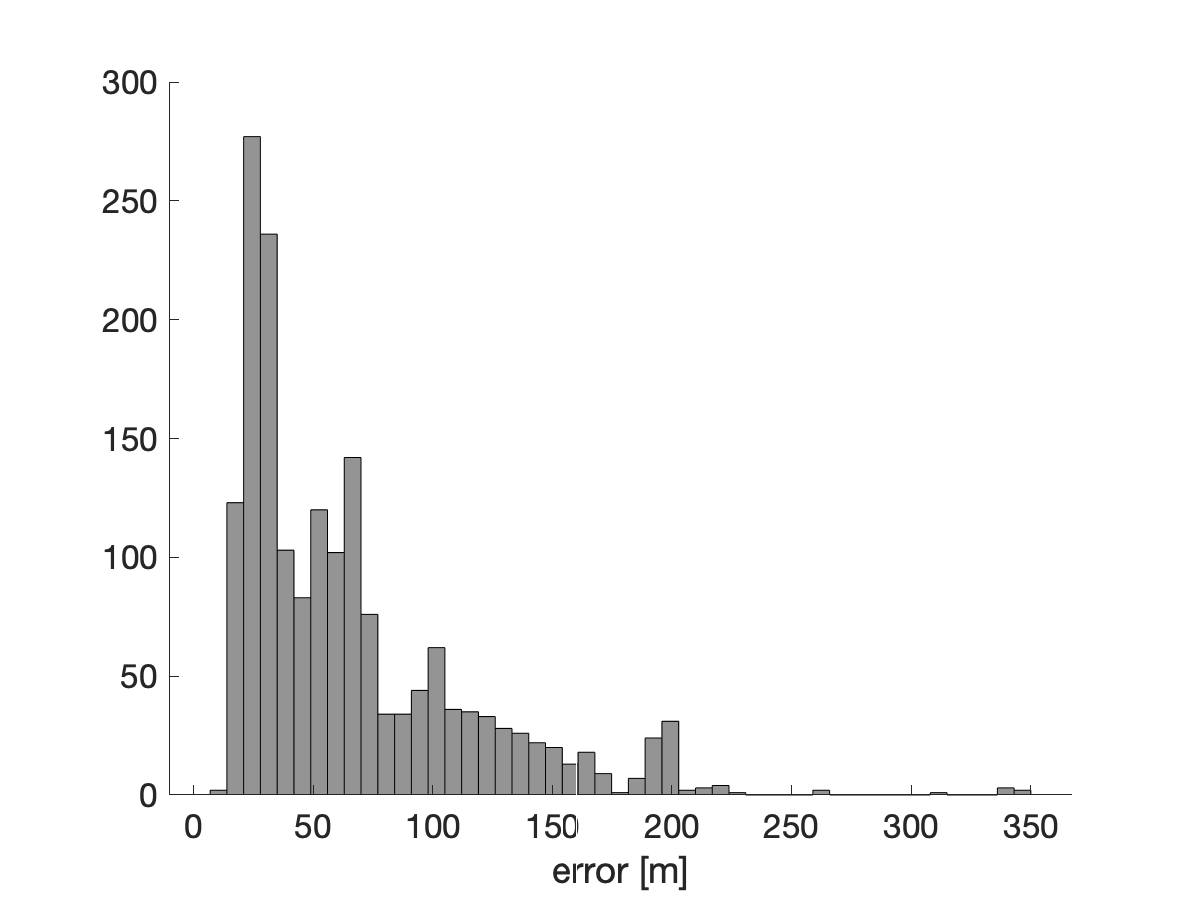
\includegraphics[width=0.3\textwidth]{kista_1}%
		\label{fig:kista_1}}
	\hfil
	\subfloat{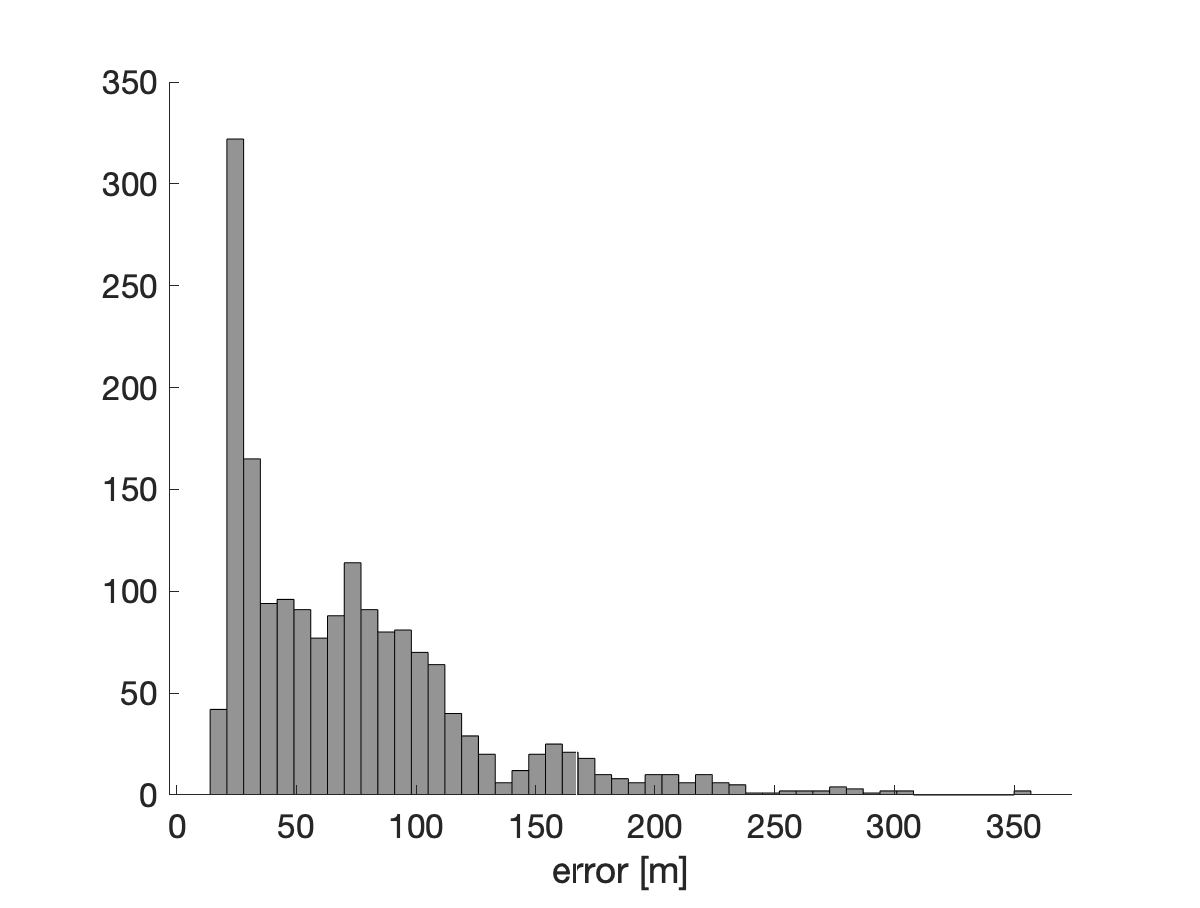
\includegraphics[width=0.33\textwidth]{kista_2}%
		\label{fig:kista_2}}
	\hfil
	\subfloat{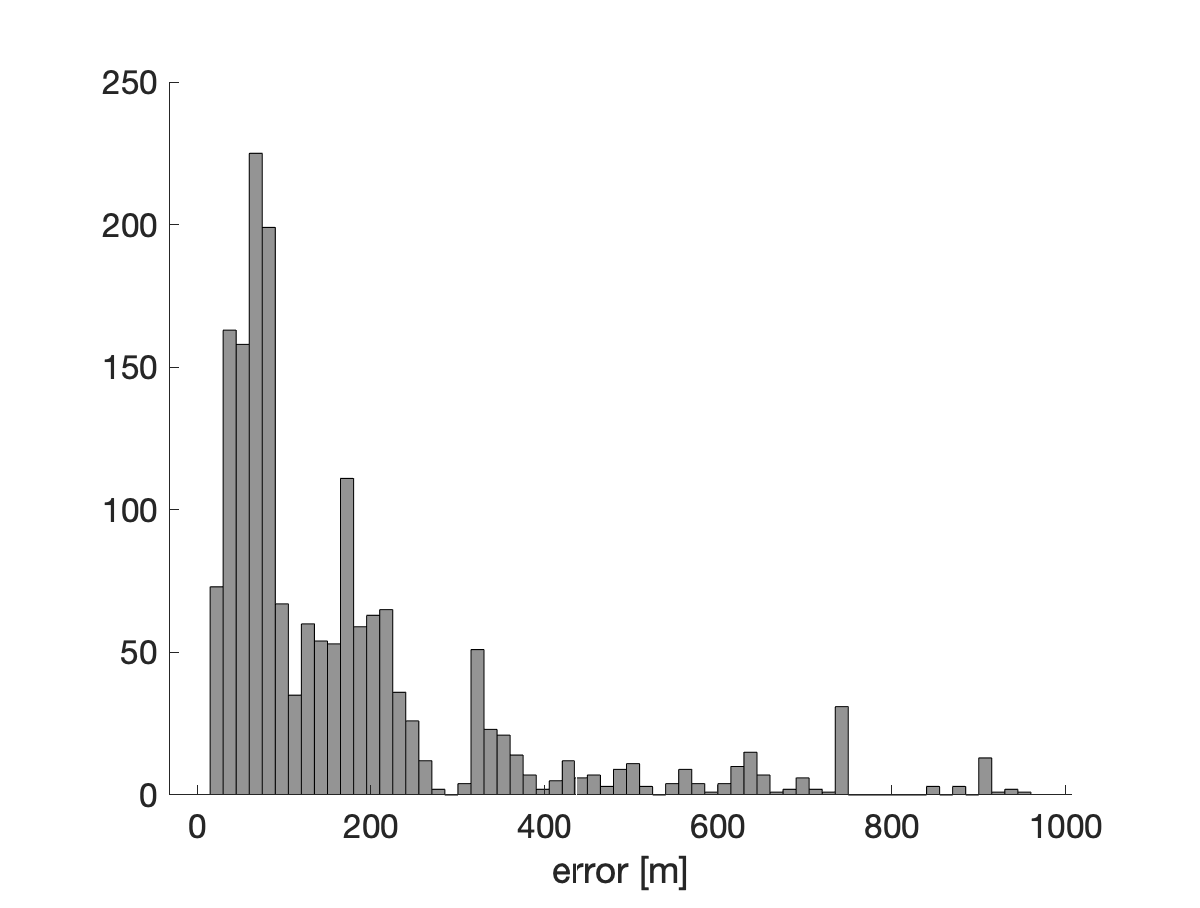
\includegraphics[width=0.33\textwidth]{kista_3}%
		\label{fig:kista_3}}	
	\caption{The error histograms of time-of-arrival measurements collected from three separate cellular antennas described in~\cite{conf:PIMRC_medbo_09}.}
	\label{fig:kista}
\end{figure*}
%
%

To deal with the estimation's performance degradation in non-Gaussian error conditions, conventional estimation techniques which are developed based on Gaussian assumptions need to be adjusted properly. As discussed in~\cite{article:ITSP_yin_13}, ``identify and discard'', ``mathematical programming'', and ``robust estimation'' are the three broad categories of estimation methods which are robust against non-Gaussian errors. Robustness of the estimator has been a concern for many years in both research~\cite{article:JASA_stigler_73} and different engineering topics ~\cite{article:PI_kassam_85,book:SDNGN_kassam,article:SIAM_stewart_99,book:NSP_arce} for a long time now. A more recent survey on this topic containing more references can be found in~\cite{article:ISPM_zoubir_12}.

The maximum likelihood estimator (MLE), developed under Gaussian assumptions, can be modified to become robust in presence of non-Gaussian noises. The authors in~\cite{conf:ICML_eskin_00} first detect and then reject the outliers by learning the PDF of the measurements and develop a mixture model of outliers and clean data. A similar idea to k-nearest-neighbor approach is used in~\cite{article:DMKD_chawla_10} to classify outliers as the data points that are less similar to a number of neighboring measurements. Surveys of advances in clustering the data into outliers and clean data can be found in~\cite{article:AIR_hodge_04,article:ITSP_yin_13,conf:ICASSP_fritsche_09}. While these approaches might result in high estimation accuracy, they typically require large datasets~\cite{article:ISPM_zoubir_12}.

M-estimators~\cite{book:RS_huber}, in the contrary to identification-based methods, do not require pre-processing and can be used in non-Gaussian noise conditions. In principle, M-estimators can be seen as generalization of MLE and rely on solving a minimization problem of some loss function. For a detailed discussion on different loss functions, see~\cite{book:RS_huber}. Since minimization problems are typically solved numerically based on the derivative of the loss function~\cite{book:RSTM_maronna}, they might converge to local minima.

In this work, we strive to find minimum variance unbiased (MVU) estimators for the location of estimation problems for non-Gaussian noise distributions where multiple distributions with positive support are considered. The most intuitive way for finding the MVU is to use Cramer-Rao lower bound (CRLB) theorem. However, the considered noise distributions do not satisfy regularity condition, hence CRLB theorem cannot be applied. Instead, we rely on  Rao-Blackwell-Lehmann-Scheffe (RBLS) theorem to find the MVU. Since the PDF cannot always be factorized in the framework of the RBLS theorem, however, we are not able to find MVU in all scenarios. In such cases, we introduce unbiased order-statistic-based estimators and compare their variances against the BLUE. Additionally, the MVU estimators without any knowledge of the hyper parameters of the noise distributions are also derived, if possible. Finally, we derive an estimator for the case in which the noise follows a mixture of normal and uniform distribution.

The rest of this paper is structured  as follows. In Section~\ref{sec:marginal_distribution_of_order_statistics} the marginal distribution of order statistics is introduced. In Section~\ref{sec:location_estimation_problem} the location estimation problem is formulated. The problem is then investigated for different noise distributions and estimators for each distribution are derived in Sections~\ref{sec:uniform_distribution}--\ref{sec:other_distributions}. The proposed estimators are evaluated in a simulation study in Section~\ref{sec:performance_evaluation} followed by the concluding remarks given in Section~\ref{sec:conclusions}.

%%%%%%%%%%%%%%%%%%%%%%%%%%%%%%%%%%%%
%---------------------------SECTION----------------------------
%%%%%%%%%%%%%%%%%%%%%%%%%%%%%%%%%%%%
\section{Marginal Distribution of Order Statistics}\label{sec:marginal_distribution_of_order_statistics}
The marginal distribution of order statistics, in this work is computed by differentiating the corresponding cumulative distribution function (CDF). In this section, we first introduce the minimum, also know as first or extreme, order statistic and then give the generalization to any statistics of order $k$. Let $F$ denote the common CDF of $N$ independent and identically distributed sample of random variables $Y_1,\ldots,Y_N$. We let $Y_{(k)}$ denote the $k$:th order statistic of the sample, defined as the $k$:th smallest value of the set $\{Y_i\}_{i=1}^N$. We define $f_{(k,N)}(y)$ as the marginal probability density function (PDF) of the $k$:th order statistics corresponding to a sample of size $N$. The PDF $f_{(k,N)}(y)$ is then calculated by differentiating $F_{(k,N)}(y)$ with respect to $y$.

%<<<<<<<<<<<<<<<<<<<<<<<<<<<<<<<<<<<<<<<<<<<<<<<<
%------------------------SUBSECTION--------------------------
%<<<<<<<<<<<<<<<<<<<<<<<<<<<<<<<<<<<<<<<<<<<<<<<<
\subsection{Marginal distribution of minimum order statistic}\label{subsec:marginal_distribution}
To further illustrate the problem, consider fist an example in which we have drawn $N=5$ independent random variables $\{Y_i\}_{i=1}^5$ each from a common distribution with PDF $f(y)$.  Assume that we are interested in the PDF of the first order statistic, $f_{(1,5)}(y)$. The CDF $F_{(1,5)}(y)$ is defined as $P(Y_{(1)} < y)$. We note that the minimum order statistic $Y_{(1)}$ would be less than $y$ if at least $1$ of the random variables $Y_1, Y_2, Y_3, Y_4, Y_5$ are less than $y$. In other words, we need to count the number of ways that can happen such that at least one random variable is less than $y$. This leads to a binomial probability calculation. The 'success' is considered to be the event $\{Y_i < y\}$, $i = 1$ and we let $\zeta$ denote the number of successes in five trials, then
%
%
\begin{align*}
F_{(1,5)}(y) &= P(Y_{(1)}<y) = P(\zeta=1)+\ldots + P(\zeta=5),\\
f_{(1,5)}(y) &= \frac{\,d}{\,dy}F_{(1,5)}(y).
\end{align*}
%
%

To generalize the example, let $Y_{(1)} < Y_{(2)} < \ldots < Y_{(N)}$ be the order statistics of $N$ independent observations from a continuous distribution with cumulative distribution function $F(y)$ and probability density function $f(y)=F'(y)$. The marginal PDF $f_{(1,N)}(y)$ of the minimum order statistic  can be obtained by considering the event $\{Y_i \leq y\}, i = 1$ as a "success," and letting $\zeta$ = the number of such successes in $N$ mutually independent trials. $\zeta$ is a binomial random variable with $N$ trials and probability of success $P(Y_i\leq y)$. Hence, the CDF of the minimum order statistic is given by,
%
%
\begin{subequations}
	\begin{align}
	F_{(1,N)}(y)=\sum_{n=1}^{N}P(\zeta=n).
	\label{eq:cdf_order_minimum}
	\end{align}
	%
	%
	Noting that the probability mass function of this binomial distribution is given by,
	\begin{align}
	P(\zeta=n) = \begin{pmatrix}N\\n\end{pmatrix}[F(y)]^n[1-F(y)]^{N-n}.
	\label{eq:pmf_order_minimum}
	\end{align}
	%
	%
	
	Substituting~\eqref{eq:pmf_order_minimum} into~\eqref{eq:cdf_order_minimum} and taking the last term out of the sum, we get 
	\begin{align}
	F_{(1,N)}(y)=\sum_{n=1}^{N-1}\begin{pmatrix}N\\n\end{pmatrix}[F(y)]^n[1-F(y)]^{N-n}+[F(y)]^N.
	\label{eq:cdf_order_minimum_2}
	\end{align}
\end{subequations}

Differentiating~\eqref{eq:cdf_order_minimum_2} with respect to $y$ gives a telescoping sum. %of the form,
%
%
%\begin{equation}
%\begin{aligned}
%f_{(1,N)}(y)= {} \lbrace&\sum_{n=1}^{N-1}\frac{N!}{(n-1)!(N-n)!}\\&\times[F(y)]^{n-1}f(y)[1-F(y)]^{N-n}\rbrace\\ &+\{ \sum_{n=1}^{N-1}\frac{N!}{n!(N-n-1)!}\\&\times[F(y)]^n[1-F(y)]^{N-n-1}(-f(y))\}\\&+ N[F(y)]^{N-1}f(y),
%\end{aligned}
%\end{equation}
%
%
in which, except the first term, all other terms cancel each other out. Hence, the marginal probability density function of the minimum order statistic of a set of $N$ independent and identically random variables with common CDF $F(y)$ and PDF $f(y)$ is given by,
%
%
\begin{align}
f_{(1,N)}(y) = Nf(y)\left(1-F(y)\right)^{N-1}.
\label{eq:density_order_minimum}
\end{align}
%
%
%<<<<<<<<<<<<<<<<<<<<<<<<<<<<<<<<<<<<<<<<<<<<<<<<
%------------------------SUBSECTION--------------------------
%<<<<<<<<<<<<<<<<<<<<<<<<<<<<<<<<<<<<<<<<<<<<<<<<
\subsection{Marginal distribution of general order statistic}\label{subsec:marginal_distribution_of_general_order_statistic}
The marginal PDF $f_{(k,N)}(y)$ of the general order statistic $k$ can be obtained by generalizing the results of the previous section, and considering the event $\{Y_i \leq y\}, i = 1, 2, \ldots, k$ as a "success," and letting $\zeta$ = the number of such successes in $N$ mutually independent trials,
%
%
\begin{align}
F_{(k,N)}(y)=\sum_{n=k}^{N-1}\begin{pmatrix}N\\n\end{pmatrix}[F(y)]^n[1-F(y)]^{N-n}+[F(y)]^N.
\label{eq:cdf_generic2}
\end{align}
%
%
Differentiating~\eqref{eq:cdf_generic2} with respect to $y$ gives a telescoping sum of the form,
%
%
\begin{equation}
\begin{aligned}
f_{(k,N)}(y)= {} \lbrace&\sum_{n=k}^{N-1}\frac{N!}{(n-1)!(N-n)!}\\&\times[F(y)]^{n-1}f(y)[1-F(y)]^{N-n}\rbrace\\ &+\{ \sum_{n=k}^{N-1}\frac{N!}{n!(N-n-1)!}\\&\times[F(y)]^n\times[1-F(y)]^{N-n-1}(-f(y))\}\\&+ N[F(y)]^{N-1}f(y),
\end{aligned}
\end{equation}
%
%
in which, except the first term, all other terms cancel each other. Hence, the marginal probability density function of the $k$:th order statistic of a set of $N$ independent and identically random variables with common CDF $F(y)$ and PDF $f(y)$ is given by,
%
%
\begin{align}
f_{(k,N)}(y) = Nf(y)\begin{pmatrix}N-1\\k-1\end{pmatrix}F(y)^{k-1}\left(1-F(y)\right)^{N-k}.
\label{eq:density_order}
\end{align}
%---------------------------SECTION----------------------------
%%%%%%%%%%%%%%%%%%%%%%%%%%%%%%%%%%%%
\section{Location Estimation Problem}\label{sec:location_estimation_problem}
Consider the location estimation problem in which we have measurements $y_k$, $k=1,\ldots,N$ of the unknown parameter $x$. The measurements are corrupted with additive noise $e_k$. The measurement model is thus given by
%
%
\begin{align}
y_k=x+e_k, \quad k=1,\ldots,N
\label{eq:original_model}
\end{align}
%
%

The best linear unbiased estimator (BLUE) for the estimation problem~\eqref{eq:original_model} is given by
%
%
\begin{align}
\hat{x}_{\mathrm{BLUE}}^{dist} &= \frac{1}{N}\sum_{k=1}^N y_k - b(\bm{y}),
\label{eq:mean_estimator}
\end{align}
%
%
where $dist$ corresponds to the particular noise distribution and $b(\bm{y})=\mathrm{E}(\frac{1}{N}\sum_{k=1}^N y_k)$ is the bias compensation term. In the following sections, closed-form expressions for the variance of the BLUE estimator for multiple noise distributions with positive support and for the are provided.  If possible, the MVU estimator for each noise distribution is derived and denoted by $\hat{x}_{\mathrm{MVU}}^{dist}$. Otherwise, an unbiased order-statistics-based estimator is derived and denoted by $\hat{x}^{dist}$. Additionally, if the hyper parameters of the distribution are assumed to be known, we parameterize the superscript {\em dist} accordingly and will ignore the parameters of the distribution otherwise. For example, $\hat{x}^{\mathcal{U}[a,b]}_{\mathrm{MVU}}$ denotes the MVU estimator when noise is uniformly distributed and $a,b$  are known. $\hat{x}^{\mathcal{U}}_{\mathrm{MVU}}$, on the other hand, corresponds to the MVU estimator of uniform noise with unknown hyper parameters of the distribution.

In order to find the MVU estimator, the first step is to find the PDF $f(\bm{y};\bm{\theta})$ with $\bm{\theta}$ denoting the parameters of the distribution. If the PDF satisfies regularity conditions, the CRLB can be determined. Any unbiased estimator that satisfies CRLB is thus the MVU estimator. However, the considered PDFs do not satisfy the regularity conditions,
%
%
\begin{align}
\E\left[\frac{\partial\ln f(y_k;\bm{\theta})}{\partial \theta}\right]\neq0.
\end{align}
%
%
Hence, the CRLB approach is not applicable. Instead, we rely on the RBLS theorem~\cite{article:IJS_lehmann_1,article:IJS_lehmann_2,book:ET_kay_93}, to find the MVU estimator. The theorem gives that for any unbiased estimator $\bar{\bm{\theta}}$ and sufficient statistics $\bm{T}(\bm{y})$, $\hat{\bm{\theta}}=\E(\tilde{\bm{\theta}}\mid\bm{T}(\bm{y}))$ is unbiased and $\Var(\hat{\bm{\theta}})\leq\Var(\tilde{\bm{\theta}})$. Additionally, if $\bm{T}(\bm{y})$ is complete, then $\hat{\bm{\theta}}$ is MVU.

As shown in~\cite{book:ET_kay_93}, if the dimension of the sufficient statistics is equal to the dimension of the parameter, then the MVU estimator is given by $\hat{\bm{\theta}}=\bm{g}(\bm{T}(\bm{y}))$ for any function $\bm{g}(\cdot)$ that satisfies
%
%
\begin{align}
\E(\bm{g}(\bm{T})) = \bm{\theta}
\end{align}
%
%
Hence, the problem of MVU estimator turns into the problem of finding a complete sufficient statistic. The Neyman-Fisher theorem~\cite{article:fisher_22,article:AMS_halmos_49} gives the sufficient statistic $\bm{T}(\bm{y})$, if the PDF can be factorized as follows
%
%
\begin{align}
f(\bm{y};\bm{\theta}) = \bm{g}(\bm{T}(\bm{y}),\bm{\theta})\bm{h}(\bm{y}).
\end{align}
%
%
%%%%%%%%%%%%%%%%%%%%%%%%%%%%%%%%%%%%
%---------------------------SECTION----------------------------
%%%%%%%%%%%%%%%%%%%%%%%%%%%%%%%%%%%%
\section{Uniform Distribution}\label{sec:uniform_distribution}
As the simplest scenario, we consider the case in which the additive noise $e_k$ in~\eqref{eq:original_model} has a uniform distribution with a positive support,$e_k\sim\mathcal{U}[0,b]$, $b>0$. The BLUE is given by,
%
%
\begin{subequations}
	\begin{align}
	\hat{x}_{\mathrm{BLUE}}^{\mathcal{U}[0,b]} &= \frac{1}{N}\sum_{k=1}^N y(k) - \frac{b}{2}.
	\label{eq:sample_mean_example}
	\end{align}
	%
	%
	The variance of BLUE for this case is given by,
	%
	%
	\begin{align}
	\Var(\hat{x}_{\mathrm{BLUE}}^{\mathcal{U}[0,b]}) &= \frac{1}{N^2}\sum_{k=1}^{N}\Var\left(y_k-\frac{b}{2}\right)= \frac{b^2}{12N}.
	\end{align}
\end{subequations}
\subsection{MVU estimator}\label{subsec:mvu_estimator}


In order to find the MVU estimator, we note that the PDF is given by,
%
%
\begin{subequations}\label{eq:uniform_pdf_1}
	\begin{align}
	f(y_k;x,b) = \left\{\begin{matrix}
	\frac{1}{b} &x< y_k< x+b \\ 
	0&\mathrm{otherwise.} 
	\end{matrix}\right.
	\end{align}
	%
	%
	that can be written in a compact form using the step function $\sigma(\cdot)$ as
	%
	%
	\begin{align}
	f(y_k;x,b) = \frac{1}{b}\left[\sigma(y_k-x) - \sigma(y_k-x-b)\right].
	\label{eq:uniform_pdf_single}
	\end{align}
	%
	%
	Since the regularity condition does not hold for~\eqref{eq:uniform_pdf_single}, the RBLS theorem is used. From~\eqref{eq:uniform_pdf_1}, we have
	%
	%
	\begin{align}
	f(\bm{y};x,b) &= \frac{1}{b^N}\prod_{k=1}^{N}\left[\sigma(y_k-x) - \sigma(y_k-x-b)\right]\nonumber\\
	&=\frac{1}{b^N}\left[\sigma(\min y_k -x) - \sigma(\max y_k -x -b)\right].%\nonumber\\
	%&=g\left(T_1(\bm{y}),T_2(\bm{y}),x\right)\cdot h(\bm{y}),
	\label{eq:unknown}
	\end{align}
\end{subequations}
%
%

The expressions for the MVU estimator is derived for two different scenarios. We first assume that the hyper parameter $b$ of the noise distribution is known and then further discuss the unknown hyper parameter case.  In the general case, let $\bm{\theta}=[x,b]^\top$, the Neyman-Fisher factorization gives $h(\bm{y})=1$ and 
%
%
\begin{align}
\bm{T}(\bm{y}) = \begin{bmatrix}
\min y_k \\ \max y_k
\end{bmatrix} = \begin{bmatrix}
T_1(\bm{y}) \\ T_2(\bm{y})
\end{bmatrix}
\label{eq:uniform_ss}
\end{align}
%
%

\subsubsection{Known hyper parameter $b$}\label{subsubsec:known_hyper_parameter_uniform}
When the maximum support of the uniform noise $b$ is known, the dimensionality of the sufficient statistic is larger than that of the parameter vector $\theta=x$. As discussed in~\cite{book:ET_kay_93}, the RBLS theorem can be extended to address this case if the form of a function $g(T_1(\bm{y}),T_2(\bm{y}))$ can be guessed that combines $T_1$ and $T_2$ into a single unbiased estimator of $\theta$. 

Let $Z = T_1(\bm{y})+T_2(\bm{y})=u+v$. Since $T_1$ and $T_2$ are dependent, 
%
%
\begin{subequations}
	\begin{align}\label{eq:dist_sum_gen}
	f_Z(z) = \int_{-\infty}^{\infty} f_{y_{(1)},y_{(N)}}(u,z-u)\,d_u,
	\end{align}
	where, as shown in~\cite{book:OS_david_04}, for $-\infty<u<v<\infty$, the joint density of two order statistics $y_{(i)}$ and $y_{(j)}$ is given by
	\begin{align}
	f_{y_{(i)},y_{(j)}}(u,v) = &\frac{N!}{(i-1)!(j-1-i)!(N-j)!}\nonumber\\&\times f_Y(u)f_Y(v)\left[F_Y(u)\right]^{i-1}\nonumber\\
	&\times\left[F_Y(v)-F_Y(u)\right]^{j-1-i}\left[1-F_Y(v)\right]^{N-j},
	\end{align}
	that for the extreme orders, $i=1$ and $j=N$ can be simplified to
	\begin{equation}\label{eq:order_joint_gen}
	f_{y_{(1)},y_{(N)}}(u,v) =
	\begin{cases}
	\begin{aligned}
	& N(N-1)\left[F_Y(v)-F_Y(u)\right]^{N-2} \\ & \times f_Y(u)f_Y(v)		\end{aligned} & \parbox[t]{4cm}{\raggedright $u<v$}\\
	0 & \parbox[t]{4cm}{\raggedright $u\geq v$}\\
	\end{cases} 
	\end{equation}
	%
	%
	Substituting~\eqref{eq:order_joint_gen} into~\eqref{eq:dist_sum_gen}, we get
	%
	%
	\begin{equation}
	f_Z(z) =
	\begin{cases}
	\frac{1}{2}Nb^{-N}(2x+2b-z)^{N-1}& \parbox[t]{3cm}{\raggedright $2x+b<z<2(x+b)$}\\
	\frac{1}{2}Nb^{-N}(z-2x)^{N-1} & \parbox[t]{4cm}{\raggedright $2x<z\leq2x+b$}\\
	0 & \parbox[t]{4cm}{\raggedright Otherwise.}\\
	\end{cases}
	\end{equation}
	%
	%
	It is trivial to show that
	\begin{align}
	\E(f_Z(z)) = 2x + b.
	\end{align}
\end{subequations}
%
%
Hence, noting that $b$ is known, the function $g(T_1(\bm{y}),T_2(\bm{y}))$ that gives an unbiased estimator should be of the form of
%
%
\begin{subequations}
	\begin{align}
	\hat{x}_{\mathrm{MVU}}^{\mathcal{U}[0,b]} &= g(T_1(\bm{y}),T_2(\bm{y})) = \nonumber\\
	& \frac{1}{2}(\min y_k + \max y_k) - \frac{b}{2}.
	\end{align}
	The variance of the MVU estimator is given by
	\begin{align}
	\Var(\hat{x}_{\mathrm{MVU}}^{\mathcal{U}[0,b]}) = \frac{b^2}{2N(N+3)+4}
	\end{align}
\end{subequations}
%
%
Clearly, the order statistics outperforms the BLUE one order of magnitude. 


%\begin{figure}[] 
%	\centering
%	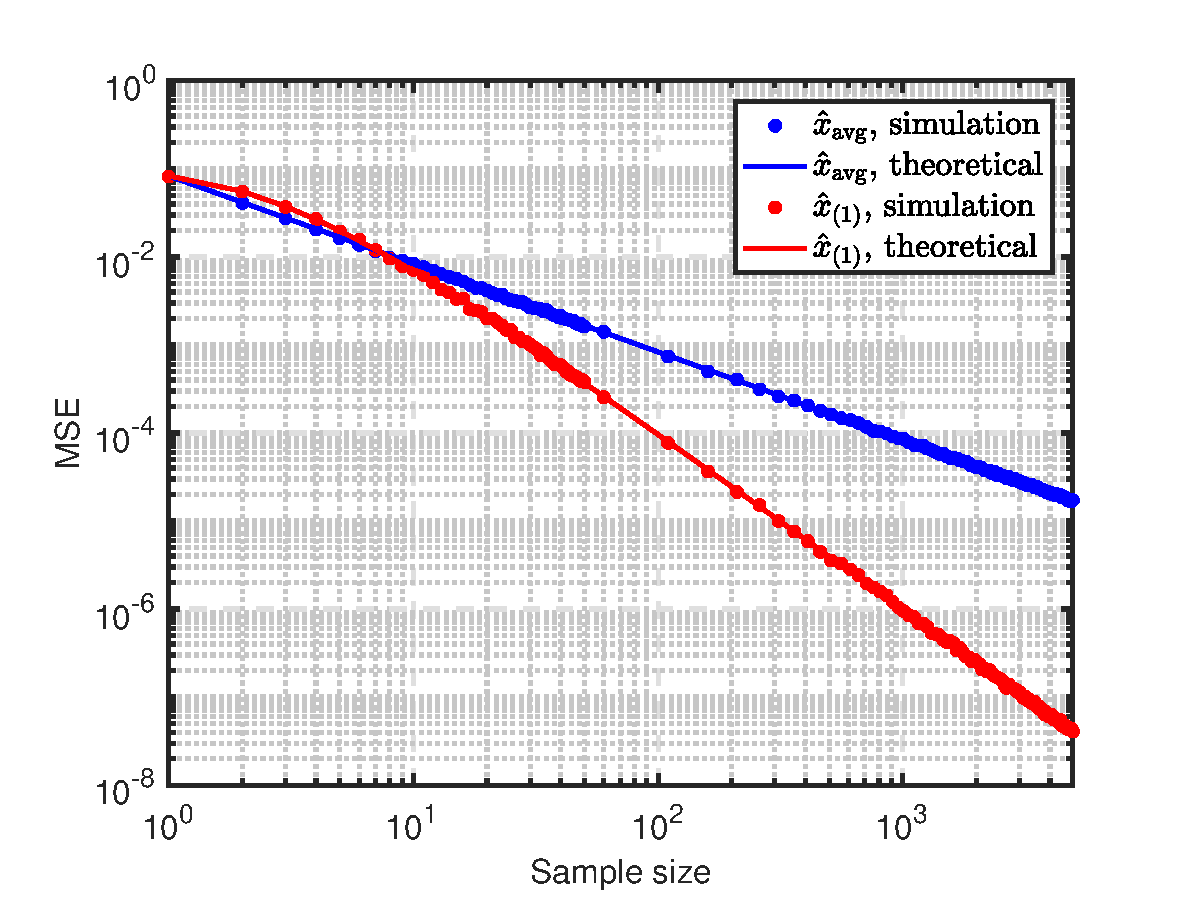
\includegraphics[width=0.7\textwidth]{mean_vs_min_Nmc5000_Nobs1-5000_uniform}
%	\caption{MSE of the sample mean~\eqref{eq:sample_mean_example} and minimum order statistic~\eqref{eq:minimum_order_example} estimators for $e\sim\mathcal{U}[0,1]$ evaluated for different sample sizes $N$. Simulated values, marked with dots, are based on 5000 Monte Carlo runs. Theoretical values are presented by solid curves. Both axes are set to logarithmic scales.}		
%	\label{fig:mean_vs_min_Nmc5000_Nobs1-5000_uniform}
%\end{figure}
%
%From the derivations above, one can conclude that if $e_k\sim\mathcal{U}[0,1]$, then the order statistic has a two-parameter beta distribution, $f_{(k,N)}^{\mathcal{U}[0,1]}(y) = \beta(k,N-k+1)$ and so has mean $\frac{k}{N+1}$ and variance $\frac{k(N-k+1)}{(N+1)^2(N+2)}$. As an illustrative example, the two estimators are compared against each other for $e_k\sim\mathcal{U}[0,1]$ in terms of their variance (MSE as they are unbiased) in a simulation study and the results are reported in Fig.~\ref{fig:mean_vs_min_Nmc5000_Nobs1-5000_uniform} in logarithmic scale. The theoretical results obtained for the bias and variance of the two estimators are also presented in Fig.~\ref{fig:mean_vs_min_Nmc5000_Nobs1-5000_uniform}. The performance of the estimators is evaluated for different sample sizes $N\in[1,5000]$. The simulation results, marked with circles, are based on $5000$ Monte Carlo runs.

%<<<<<<<<<<<<<<<<<<<<<<<<<<<<<<<<<<<<<<<<<<<<<<<<
%------------------------SUBSECTION--------------------------
%<<<<<<<<<<<<<<<<<<<<<<<<<<<<<<<<<<<<<<<<<<<<<<<<
\subsubsection{Unknown hyper parameter $b$}\label{subsec:unknown_hyper_parameter_uniform}
In this case, the MVU estimators for the parameter vector $\bm{\theta}=[x,b]$ can be derived from sufficient statistics~\eqref{eq:uniform_ss},
%
%
\begin{align}
\hat{\bm{\theta}}=\bm{g}(\bm{T}(\bm{y})),\quad \mathrm{s.t.}\quad \E\left(\bm{g}\left(\bm{T}(\bm{y})\right)\right) = \bm{\theta}.
\end{align}
%
%
Hence, we first need to find the moments of minimum and maximum order statistics.  Let $\tilde{y}_k = \frac{1}{b}y_k$. Since $y_k\sim\mathcal{U}[x,x+b]$, then for any constant $b>0$, $\tilde{y_k}\sim\mathcal{U}[\frac{x}{b},\frac{x}{b}+1]$. Hence, $f(\tilde{y}_k)=1$ and $F(\tilde{y}_k)=\frac{1}{b}(y_k-x)$. From~\eqref{eq:density_order} we get,
%
%
\begin{subequations}
	\begin{align}
	f_{(k,N)}^{\mathcal{U}[0,b]}(\tilde{y}) &= N\begin{pmatrix}N-1\\k-1\end{pmatrix}\left(\frac{y-x}{b}\right)^{k-1}\left(\frac{b-(y-x)}{b}\right)^{N-k}\nonumber\\
	&= \frac{(N)!}{(k-1)!(N-k)!}\left(\frac{y-x}{b}\right)^{k-1}\left(\frac{b-(y-x)}{b}\right)^{N-k}.
	\end{align}
	%
	%
	since $N\in\mathbb{N}^+$, $k\in\mathbb{N}^+$, and $k\in[1,N]$ we can use the change the factorials to gamma functions,
	%
	%
	\begin{align}
	f_{(k,N)}^{\mathcal{U}[0,b]}(\tilde{y}) &= \left(\frac{y-x}{b}\right)^{k-1}\left(\frac{b-(y-x)}{b}\right)^{N-k}\nonumber\\&\times\frac{\Gamma(N+1)}{\Gamma(k)\Gamma(N-k+1)}.
	\label{eq:order_uniform_general}
	\end{align}
	%
	%
\end{subequations}
%
%
The marginal distribution~\eqref{eq:order_uniform_general} is a generalized beta distribution, also known as four parameters beta distribution. The support of this distribution is from $0$ to $b>0$ and $f_{(k,N)}^{\mathcal{U}[0,b]}(\cdot)=\frac{1}{b}f_{(k,N)}^{\mathcal{U}[0,1]}(\cdot)$. Hence, the bias and variance of the order statistic estimator $y_{(k)}$ in case of uniform noise with support on $[0,b]$ are given by
%
%
\begin{subequations}
	\begin{align}
	\E(y_{(k)}^{\mathcal{U}[0,b]}) &= \frac{bk}{N+1},\\
	\Var(y_{(k)}^{\mathcal{U}[0,b]}) &= \frac{k(N-k+1)b^2}{(N+1)^2(N+2)}.
	\end{align}	
\end{subequations}
%
%
That is, 
%
%
\begin{align}
\E(\bm{T}(\bm{y})) = \begin{bmatrix}
x+\frac{b}{N+1}\\\\x+\frac{Nb}{N+1}
\end{bmatrix}
\label{eq:uniform_unknown_E_gen}
\end{align}
%
%
To find the transformation that makes~\eqref{eq:uniform_unknown_E_gen} unbiased, 
%
%
\begin{subequations}
	\begin{align}
	\bm{g}(\bm{T}(\bm{y}))=\begin{bmatrix}\frac{1}{N-1}\left(NT_1(\bm{y})-T_2(\bm{y})\right)\\\\	\frac{N+1}{N-1}\left(T_2(\bm{y})-T_1(\bm{y})\right)\end{bmatrix}
	\end{align}
	that gives
	\begin{align}
	\E\left(\bm{g}(\bm{T}(\bm{y}))\right) = \begin{bmatrix}x\\b	\end{bmatrix}
	\end{align}
\end{subequations}
Finally, the MVU estimator of $x$ when the hyper parameter $b$ is unknown is given by
\begin{subequations}
	\begin{align}
	\hat{x}_{\mathrm{MVU}}^{\mathcal{U}} = \frac{N}{N-1}\min y_k - \frac{1}{N-1} max y_k 
	\end{align}
	and its variance is
	\begin{align}
	\Var(\hat{x}_{\mathrm{MVU}}^{\mathcal{U}}) = \frac{Nb^2}{(N+2)(N^2-1)}
	\end{align}
\end{subequations}
%
%


%%%%%%%%%%%%%%%%%%%%%%%%%%%%%%%%%%%%
%---------------------------SECTION----------------------------
%%%%%%%%%%%%%%%%%%%%%%%%%%%%%%%%%%%%
\section{Distributions in the exponential family} \label{sec:distributioons_in_the_exponential_family}
% Beta and Gamma distributions, in their general form, do not give a closed-form solution for the bias and variance. However, there are other continuous non-negative distributions for which the analytical solutions exists. In this section we investigate such distributions and show that the marginal distribution of the minimum order statistic has the same "form" of distribution as the noise.
% Multiple distributions with positive support have been tested.

The exponential family of probability distributions, in their most general form are defined by,
%
%
\begin{align}
f(y;\theta) = h(y)g(\theta)\exp\left\{A(\theta)\cdot T(y)\right\},
\end{align}
%
%
where $\theta$ is the parameter of the distribution, and $h(y)$, $g(\theta)$, $A(\theta)$, and $T(y)$ are all known functions. In this section, we only consider some example distributions of this family and show that the minimum order statistic estimator gets the same form of distribution as the noise distribution but with modified parameters.
%Note that, in all distributions of the exponential family, the support of $f(y;\theta)$ does not depend on $\theta$. This excludes Pareto distribution, that will be discussed in the next section, from the exponential family. 
%<<<<<<<<<<<<<<<<<<<<<<<<<<<<<<<<<<<<<<<<<<<<<<<<
%------------------------SUBSECTION--------------------------
%<<<<<<<<<<<<<<<<<<<<<<<<<<<<<<<<<<<<<<<<<<<<<<<<  
\subsection{Exponential distribution} \label{subsec:exponential_distribution}
Exponential distributions are members of the gamma family with shape parameter 1; strongly skewed with no left sided tail ($y_k\in[x,\infty]$). Let $\beta>0$ denote the scale parameter, the PDF of an exponential distribution is then given by
%
%
\begin{subequations}\label{eq:exponential}
	\begin{align}
	f^{\mathrm{Exp}}(y_k;x,\beta)=\left\{\begin{matrix}
	\frac{1}{\beta}\exp(-\frac{(y-x)}{\beta})&y_k\geq x, \\ 
	0&y_k< x. 
	\end{matrix}\right.
	\label{eq:exponential_pdf}
	\end{align}
	%
	%
	and the CDF, for $y\geq x$, is given by
	%
	%
	\begin{align}
	F^{\mathrm{Exp}}(y_k;x,\beta)=1-\exp(-\frac{(y_k-x)}{\beta}).
	\label{eq:exponential_cdf}
	\end{align}
	%
	%
\end{subequations}

For the BLUE estimator~\eqref{eq:mean_estimator}, from the properties of exponential distribution, we have
%
%
\begin{align}
\hat{x}_{\mathrm{BLUE}}^{\mathrm{Exp}} = &= \frac{1}{N}\sum_{k=1}^{N}y_k - \beta,
&\quad 
\mathrm{Var}(\hat{x}_{\mathrm{BLUE}}^{\mathrm{Exp}}) &= \frac{\beta^2}{N}.
\end{align}
%
%
In order to find the MVU estimator, we re-write the PDF as
%
%
\begin{align}
f(\bm{y};x,\beta) &= \frac{1}{\beta^N}\exp\left[-\frac{1}{\beta}\sum_{k=1}^{N}y_k\right]\exp\left[-\frac{N}{\beta}x\right]\nonumber\\&\times\sigma(\min y_k - x)
\label{eq:exponential_pdf_2}
\end{align}
%
%
\subsubsection{Known hyper parameter $\beta$}
In this case, the Neyman-Fisher factorization of PDF~\eqref{eq:exponential_pdf_2} gives
%
%
\begin{subequations}
	\begin{align}
	T(\bm{y}) &= \min y_k\\
	h(\bm{y}) &=   \frac{1}{\beta^N}\exp\left[-\frac{1}{\beta}\sum_{k=1}^{N}y_k\right]
	\label{eq:exponential_known_ss}
	\end{align}
\end{subequations}
%
%
The MVU estimator can then be obtained from a transformation of the minimum order statistic that makes it an unbiased estimator. Substituting~\eqref{eq:exponential} into~\eqref{eq:density_order}, the marginal density of the $k$:th order statistic is given by
%
%
\begin{align}
f^{\mathrm{Exp}}_{(k,N)}(y;x,\beta) &= \frac{N}{\beta}\begin{pmatrix}N-1\\k-1\end{pmatrix}\left(1-\exp(-\frac{(y-x)}{\beta})\right)^{k-1}\nonumber\\&\times\exp\left(-\frac{(N-k+1)(y-x)}{\beta}\right).
\label{eq:exponential_order}
\end{align}
%
%

The first order statistic density is then given by letting $k=1$ in~\eqref{eq:exponential_order} that results in another exponential distribution,
%
%
\begin{align}
f^{\mathrm{Exp}}_{(1,N)}(y;x,\bar{\beta}) = f^{\mathrm{Exp}}(y;x,\beta),
\end{align}
%
%
where $\bar{\beta}=\frac{\beta}{N}$. Finally, in case of exponential noise with known hyper parameter pf the distribution, the MVU estimator and its variance are given by
%
%
\begin{align}
\hat{x}_{MVU}^{\mathrm{Exp}(\beta)} &= \min y_k - \frac{\beta}{N},
&\quad 
\mathrm{Var}(\hat{x}_{MVU}^{\mathrm{Exp}(\beta)}) &= \frac{\beta^2}{N^2}.
\end{align}
%
%
\subsubsection{Unknown hyper parameter $\beta$}
If the hyper parameter $\beta$ is unknown, the factorization gives
\begin{subequations}
	%
	%
	\begin{align}
	\bm{T}(\bm{y}) = \begin{bmatrix}
	\min y_k \\ \sum_{k=1}^{N} y_k
	\end{bmatrix} = \begin{bmatrix}
	T_1(\bm{y}) \\ T_2(\bm{y})
	\end{bmatrix}
	\label{eq:uniform_unknown_ss}
	\end{align}
	%
	% 
	Noting that sum of exponential random variables results in a Gamma distribution, we have $T_2(\bm{y})\sim\Gamma(n,\beta)$. Hence,
	%
	%
	\begin{align}
	\E(\bm{T}(\bm{y})) = \begin{bmatrix}
	x+\frac{\beta}{N}\\\\N(x+\beta)
	\end{bmatrix}
	\label{eq:exponential_unknown_E_gen}
	\end{align}
	%
	%
\end{subequations}

Following the same line of reasoning as in Section~\ref{subsec:unknown_hyper_parameter_uniform}, the unbiased estimator is given by the transformation
%
%
\begin{subequations}
	\begin{align}
	\bm{g}(\bm{T}(\bm{y}))=\begin{bmatrix}\frac{1}{N-1}\left(NT_1(\bm{y})-\frac{1}{N}T_2(\bm{y})\right)\\\\	\frac{1}{N-1}\left(T_2(\bm{y})-NT_1(\bm{y})\right)\end{bmatrix}
	\end{align}
	that gives
	\begin{align}
	\E\left(\bm{g}(\bm{T}(\bm{y}))\right) = \begin{bmatrix}x\\\beta	\end{bmatrix}
	\end{align}
\end{subequations}
Finally, the MVU estimator of $x$ when the hyper parameter $\beta$ is unknown is given by,
\begin{subequations}
	\begin{align}
	\hat{x}_{\mathrm{MVU}}^{\mathrm{Exp}} &= \frac{N}{N-1}\min y_k - \frac{1}{N(N-1)} \sum_{k=1}^{N} y_k \nonumber\\&= \frac{N}{N-1}\min y_k - \frac{1}{N-1} \bar{y} 
	\end{align}
	where $\bar{y}$ is the sample mean. Assuming that $N$ is large $\min y_k$ and $\bar{y}$ are independent and the variance of the estimator is given by
	\begin{align}
	\Var(\hat{x}_{\mathrm{MVU}}^{\mathrm{Exp}}) = \frac{\beta^2(N+1)}{N(N-1)^2}
	\end{align}
\end{subequations}
%
%
%<<<<<<<<<<<<<<<<<<<<<<<<<<<<<<<<<<<<<<<<<<<<<<<<
%------------------------SUBSECTION--------------------------
%<<<<<<<<<<<<<<<<<<<<<<<<<<<<<<<<<<<<<<<<<<<<<<<<
\subsection{Rayleigh distribution} \label{subsec:rayleigh_distribution}
One generalization of the exponential distribution is obtained by parameterizing in terms of both a scale parameter $\beta$ and a shape parameter $\alpha$. Rayleigh distribution is a special case obtained by setting $\alpha=2$
\begin{subequations}\label{eq:rayleigh}
	\begin{align}
	f^{\mathrm{Rayleigh}}(y_k;x,\beta)=\left\{\begin{matrix}
	\frac{y_k-x}{\beta^2}\exp(-\frac{(y_k-x)^2}{2\beta^2})&y_k> x, \\ 
	0&y_k\leq x. 
	\end{matrix}\right.
	\label{eq:rayleigh_pdf}
	\end{align}
	%
	%
	and the CDF, for $y_k>x$ is given by
	%
	%
	\begin{align}
	F^{\mathrm{Rayleigh}}(y_k;x,\beta)=1-\exp(-\frac{(y_k-x)^2}{2\beta^2}).
	\label{eq:rayleigh_cdf}
	\end{align}
	%
	%
\end{subequations}
Hence, the BLUE estimator~\eqref{eq:mean_estimator}, becomes
%
%
\begin{subequations}
\begin{align}
\hat{x}_{\mathrm{BLUE}}^{\mathrm{Rayleigh}(\beta)} &= \frac{1}{N}\sum_{k=1}^{N}y_k - \sqrt{\frac{\pi}{2}}\beta,
\\
\mathrm{Var}(\hat{x}^{\mathrm{Rayleigh}(\beta)}_{\mathrm{BLUE}}) &= \frac{(4-\pi)\beta^2}{2N}.
\end{align}
\end{subequations}
%
%
The joint PDF of $N$ independent observations $y_k$, $k=1,\ldots,N$ is given by
%
%
\begin{subequations}\label{eq:rayleigh_pdf_2}
	%
	%
	\begin{align}
	f(\bm{y};x,\beta) &= \frac{\prod_{k=1}^{N}(y_k-x)}{\beta^{2N}}\exp\left[\sum_{k=1}^{N}-\frac{(y_k-x)^2}{2\beta^2}\right]\nonumber\\&\times\sigma(\min y_k - x)
	\label{eq:rayleigh_pdf_2_1}
	\end{align}
	%
	%
	Noting that
	%
	%
	\begin{align}
	\sum_{k=1}^{N}(y_k-x)^2 = \sum_{k+1}^{N}y_k^2 - 2x\sum_{k=1}^{N}y_k+Nx^2
	\label{eq:rayleigh_pdf_2_2}
	\end{align}
	%
	%
	the PDF becomes
	%
	%
	\begin{align}
	f(\bm{y};x,\beta) &= \beta^{-2N}\prod_{k=1}^{N}(y_k-x)\exp\left[\frac{-1}{2\beta^2}\sum_{k=1}^{N}y_k^2\right]\nonumber\\&\times\exp\left[-\frac{Nx^2}{2\beta^2}\right]\exp\left[\frac{x}{\beta^2}\sum_{k=1}^{N}y_k\right]\sigma(\min y_k - x)
	\label{eq:rayleigh_pdf_2_3}
	\end{align}
	%
	%
\end{subequations}
%
%
\subsubsection{Known hyper parameter $\beta$}
Since~\eqref{eq:rayleigh_pdf_2_3} cannot be factorized in the form of $f(\bm{y};x,\beta) = g(T(\bm{y}),x)h(\bm{y})$, the RBLS theorem cannot be used. Additionally, as~\eqref{eq:rayleigh_pdf_2_3} is non-differentiable, CRLB theorem is not applicable either. Hence, even if a MVU estimator exists for this problem, we may not be able to find it. Thus, in case of Rayleigh-distributed measurement noise, we only provide unbiased estimators based on order statistics. 

The marginal density of the $k$:th order statistic for $y>x$ is given by
%
%
\begin{align}
f^{\mathrm{Rayleigh}}_{(k,N)}(y;x,\beta) &=
\frac{Ny}{\beta^2}\begin{pmatrix}N-1\\k-1\end{pmatrix}\left(1-\exp(-\frac{(y-x)^2}{2\beta^2})\right)^{k-1}\nonumber\\&\times\exp\left(-\frac{(N-k+1)(y-x)^2}{2\beta^2}\right).
\label{eq:rayleigh_order}
\end{align}
%
%
Hence, the minimum order statistics density has also Rayleigh distribution 
%
%
\begin{align}
f^{\mathrm{Rayleigh}}_{(1,N)}(y;x,\bar{\beta}) = f^{\mathrm{Rayleigh}}(y;x,\beta),
\end{align}
%
%
where $\bar{\beta}=\frac{\beta}{\sqrt{N}}$.  The minimum order statistic unbiased estimator $\hat{x}^{\mathrm{Rayleigh}(\beta)}$ is then given by,
%
%
\begin{subequations}
\begin{align}
\hat{x}^{\mathrm{Rayleigh}(\beta)} &= \min y_k - \frac{\sqrt{\pi}\beta}{\sqrt{2N}},
\\ 
\Var(\hat{x}^{\mathrm{Rayleigh}(\beta)}) &=\frac{(4-\pi)\beta^2}{2N}.
\end{align}
\end{subequations}
%
%
which has the same variance as the BLUE estimator.
\subsubsection{Unknown hyper parameter $\beta$}
As in the case of known hyper parameter, the RBLS theorem cannot be applied for this case either and the MVU estimator, even if exists, cannot be found. In order to compensate for the bias, however, we need to combine two estimators.  We propose the following unbiased estimator
%
%
\begin{align}
\hat{x}^{\mathrm{Rayleigh}} = \min y_k - \frac{1}{N\sqrt{N}}\sum_{k=1}^{N}y_k = \min y_k - \frac{1}{\sqrt{N}}\bar{y}.
\end{align}
%
% 
Asymptotically, for large $N$ the sample mean and minimum order statistic are independent and the estimator variance is given by
%
%
\begin{align}
\Var(\hat{x}^{\mathrm{Rayleigh}})=\frac{(1+N)(4-\pi)\beta^2}{2N^2}
\label{eq:minimum_orde_unknown_rayleigh}
\end{align}
%
%
%<<<<<<<<<<<<<<<<<<<<<<<<<<<<<<<<<<<<<<<<<<<<<<<<
%------------------------SUBSECTION--------------------------
%<<<<<<<<<<<<<<<<<<<<<<<<<<<<<<<<<<<<<<<<<<<<<<<<
\subsection{Weibull distribution} \label{subsec:weibull_distribution}
Weibull distribution is a generalization of the Rayleigh, and hence exponential, distributions that is parametrized by teo parameters--scale parameter $\beta$ and shape parameter $\alpha>0$. In fact Weibull distribution is obtained by relaxing the assumption $\alpha=2$ in the Rayleigh distribution and its density function for $y>x$ is given by
%
%
\begin{subequations}\label{eq:weibull}
	\begin{align}
	f^{\mathrm{Weibull}}(y_k;x,\beta,\alpha)=
	\frac{\alpha}{\beta}\left(\frac{y_k-x}{\beta}\right)^{\alpha-1}\exp(-(\frac{y_k-x}{\beta})^\alpha)
	\label{eq:weibull_pdf}
	\end{align}
	%
	%
	and the CDF, for $y_k\geq x$ is given by
	%
	%
	\begin{align}
	F^{\mathrm{Weibull}}(y_k;x,\beta,\alpha)=1-\exp(-(\frac{y_k-x}{\beta})^\alpha).
	\label{eq:weibull_cdf}
	\end{align}
\end{subequations}
	%
	%
	The BLUE estimator, in case of Weibull-distributed measurement noises is given by
	%
	%
	\begin{subequations}
			\begin{align}
		\hat{x}_{\mathrm{BLUE}}^{\mathrm{Weibull}(\beta,\alpha)} &= \frac{1}{N}\sum_{k=1}^{N}y_k - \beta\Gamma(1+\frac{1}{\alpha}),
		\\
		\mathrm{Var}(\hat{x}_{\mathrm{BLUE}}^{\mathrm{Weibull}(\beta,\alpha)}) &= \frac{\beta^2}{N}\left[\Gamma(\frac{\alpha+2}{\alpha})-\left(\Gamma(\frac{\alpha+1}{\alpha})\right)^2\right].
		\end{align}
	\end{subequations}
	%
	%
Given $N$ independent observations, the joint density is given by
%
%
\begin{align}
f^{\mathrm{Weibull}}(\bm{y};x,\beta,\alpha)&=(\frac{\alpha}{\beta})^N\prod_{k=1}^{N}\left(\frac{y_k-x}{\beta}\right)^{\alpha-1}\nonumber\\&\times\exp(-\sum_{k=1}^{N}(\frac{y_k-x}{\beta})^\alpha)\sigma(\min y_k - x)
\label{eq:weibull_pdf_joint}
\end{align}
%
%
Since~\eqref{eq:weibull_pdf_joint} cannot be factorized using Neyman-Fisher factorization, RBLS is not applicable. Additionally, in this case, it is not possible to find an unbiased estimator when the hyper parameters $\alpha$ and $\beta$ are unknown. In case of known hyper parameters, the unbiased minimum order statistic estimator, however, can be computed.  For this purpose, we first compute the marginal density of the $k^{\mathrm{th}}$ order statistic
%
%
\begin{align}
f^{\mathrm{Weibull}}_{(k,N)}(y;x,\beta,\alpha) &= \frac{N\alpha}{\beta}\begin{pmatrix}N-1\\k-1\end{pmatrix}(\frac{y-x}{\beta})^{\alpha-1}\nonumber\\&\times\left(1-\exp^{-(\frac{y-x}{\beta})^\alpha}\right)^{k-1}\nonumber\\&\times\exp\left(-(N-k+1)(\frac{y-x}{\beta})^\alpha\right).
\label{eq:weibull_order}
\end{align}
%
%

%
%
Hence, the first order statistic density in case of $e_k\sim\mathrm{Weibull}(\beta,\alpha)$, is another Weibull distribution,
%
%
\begin{align}
f^{\mathrm{Weibull}}_{(1,N)}(y;x,\bar{\beta},\alpha) = f^{\mathrm{Weibull}}(y;x,\beta,\alpha),
\end{align}
%
%
where $\bar{\beta}=\sqrt[-\alpha]{N}\beta$. The unbiased estimator based on minimum order statistic is then given by,
%
%
\begin{subequations}
\begin{align}
\hat{x}^{\mathrm{Weibull}(\beta,\alpha)} = &= \min_y y_{1:N} - \beta N^{-\frac{1}{\alpha}}\Gamma(1+\frac{1}{\alpha}),
\\
\Var(\hat{x}^{\mathrm{Weibull}(\beta,\alpha)}) &=\beta^2N^{\frac{-2}{\alpha}}\left[\Gamma(\frac{\alpha+2}{\alpha})-\left(\Gamma(\frac{\alpha+1}{\alpha})\right)^2\right].
\end{align}
\end{subequations}
%
%
An order-statistics-based unbiased estimator with unknown hyper parameters of the distribution could not be obtained.
\begin{table*}[h]
	\centering
	\caption{Estimators and their variances derived for multiple noise distributions.}
	\resizebox{\textwidth}{!}{
		\begin{tabular}{c|l|l|cl}
			\hline
			\begin{tabular}[c]{@{}c@{}}noise\\ distribution\end{tabular} &
			\multicolumn{2}{c|}{estimator}                                                                                            & \multicolumn{2}{c}{variance}                                                                                                         \\  \hline
			\multirow{3}{*}{\vspace{-6mm}$\mathcal{U}[0,b]$}                          & \multicolumn{2}{l|}{$\hat{x}_\mathrm{BLUE} = \frac{1}{N}\sum y_k - \frac{b}{2}$}                                          &   \multicolumn{2}{c}{$\frac{b^2}{12N}$}                                                                                                 \\[2mm] 
			& \multicolumn{2}{l|}{known b: $\hat{x}_\mathrm{MVU} = \frac{1}{2}(\min y_k + \max y_k) - \frac{b}{2}$}                     & \multicolumn{2}{c}{$\frac{b^2}{2N(N+3)+4}$}                                                                                           \\[2mm] 
			& \multicolumn{2}{l|}{unknown b: $\hat{x}_\mathrm{MVU} = \frac{N}{N-1}\min y_k - \frac{1}{N-1} \max y_k$}                   & \multicolumn{2}{c}{$\frac{Nb^2}{(N+2)(N^2-1}$}                                                                                        \\[2mm]  \hline
			\multirow{3}{*}{\vspace{-6mm}$\mathrm{Exp}(\beta)$}                       & \multicolumn{2}{l|}{$\hat{x}_\mathrm{BLUE} = \frac{1}{N}\sum y_k -\beta$}                                                 & \multicolumn{2}{c}{$\frac{\beta^2}{N}$}                                                                                             \\[2mm]
			& \multicolumn{2}{l|}{known $\beta$: $\hat{x}_\mathrm{MVU} = \min y_k - \frac{\beta}{N}$}                                   & \multicolumn{2}{c}{$\frac{\beta^2}{N^2}$}                                                                                           \\[2mm]
			& \multicolumn{2}{l|}{unknown $\beta$: $\hat{x}_\mathrm{MVU} = \frac{N}{N-1}\min y_k - \frac{1}{N(N-1)}\sum y_k$}           & \multicolumn{2}{c}{$\frac{(N+1)\beta^2}{N(N-1)^2}$}                                                                                 \\[2mm] \hline
			\multirow{3}{*}{\vspace{-6mm}$\mathrm{Rayleigh}(\beta)$}                  & \multicolumn{2}{l|}{$\hat{x}_\mathrm{BLUE} = \frac{1}{N}\sum y_k -\sqrt{\frac{\pi}{2}}\beta$}                             & \multicolumn{2}{c}{$\frac{(4-\pi)\beta^2}{2N}$}                                                                                     \\[2mm]
			& \multicolumn{2}{l|}{known $\beta$: $\hat{x} = \min y_k - \frac{\sqrt{\pi}\beta}{\sqrt{2N}}$}                              & \multicolumn{2}{c}{$\frac{(4-\pi)\beta^2}{2N}$}                                                                                      \\[2mm]
			& \multicolumn{2}{l|}{unknown $\beta$: $\hat{x} = \min y_k - \frac{1}{N\sqrt{N}}\sum y_k$}                                  & \multicolumn{2}{c}{$\frac{(1+N)(4-\pi)\beta^2}{2N^2}$}                                                                               \\[2mm] \hline
			\multirow{2}{*}{\vspace{-4mm}$\mathrm{Weibull}(\beta,\alpha)$}            & \multicolumn{2}{l|}{$\hat{x}_\mathrm{BLUE} = \frac{1}{N}\sum y_k -\beta \Gamma(1+\frac{1}{\alpha})$}                      & \multicolumn{2}{c}{$\beta^2 N^{-1}\left[\Gamma(1+\frac{2}{\alpha})-\left(\Gamma(1+\frac{1}{\alpha})\right)^2\right]$}               \\[2mm]
			& \multicolumn{2}{l|}{ known $\beta$, $\alpha$: $\hat{x} = \min y_k - \beta N^{-\frac{1}{\alpha}}\Gamma(1+\frac{1}{\alpha})$} & \multicolumn{2}{c}{$\beta^2 N^{-\frac{2}{\alpha}}\left[\Gamma(1+\frac{2}{\alpha})-\left(\Gamma(1+\frac{1}{\alpha})\right)^2\right]$} \\[2mm] \hline
			\multirow{2}{*}{\vspace{-3mm}$\mathrm{Pareto}(\beta,\alpha)$}             & \multicolumn{2}{l|}{$\hat{x}_\mathrm{BLUE} = \frac{1}{N}\sum y_k -\frac{\alpha\beta}{\alpha-1}$, $\alpha>1$}              & \multicolumn{2}{c}{$\frac{\alpha\beta^2}{N(\alpha -1)^2(\alpha -2)}$, $\alpha>2$}                                                     \\[2mm]
			& \multicolumn{2}{l|}{known $\beta$, $\alpha$: $\hat{x} = \min y_k - \frac{N\alpha\beta}{N\alpha -1}$, $N\alpha>1$}         & \multicolumn{2}{c}{$\frac{N\alpha\beta^2}{(N\alpha -1)^2(N\alpha -2)}$}                                                             
			\\[2mm] \hline
			\multirow{2}{*}{$a\mathcal{N}(0,\sigma^2) + (1-a)\mathcal{U}(0,b)$}             & \multicolumn{2}{l|}{$\hat{x}_\mathrm{MLE} =y_{(\lfloor\frac{Na}{2}\rfloor+1)}$}
			& \multicolumn{2}{c}{-} \\[3mm]  \hline
	\end{tabular}}
	\label{tbl:estimators}
\end{table*}
\section{Other Distributions}\label{sec:other_distributions}
In this section, we further study the location estimation problem for two other noise distributions. In the rest, the Pareto distribution with positive support is first studied followed by the mixture of uniform and normal distribution.

\subsection{Pareto distribution} 
Let the scale parameter $\beta$ (necessarily positive) denote the minimum possible value of $y_k$, and $\alpha>0$ denote the shape parameter. The Pareto Type I distribution is characterized by $\beta$ and $\alpha$
%
%
\begin{subequations}\label{eq:pareto}
	\begin{align}
	f^{\mathrm{Pareto}}(y_k;x,\beta,\alpha)=\left\{\begin{matrix}
	\alpha\beta^\alpha (y-x)^{-(\alpha+1)}&y\geq x+\beta, \\ 
	0&y< x+\beta. 
	\end{matrix}\right.
	\label{eq:pareto_pdf}
	\end{align}
	%
	%
	and the CDF is given by
	%
	%
	\begin{align}
	F^{\mathrm{Pareto}}(y_k;x,\beta,\alpha)=1-\left(\frac{\beta}{y-x}\right)^\alpha.
	\label{eq:pareto_cdf}
	\end{align}
	%
	%
\end{subequations}
%
%
For the BLUE we get,
%
%
\begin{subequations}
	\begin{align}
	\hat{x}_{\mathrm{BLUE}}^{\mathrm{Pareto}(\beta,\alpha)} = &= \frac{1}{N}\sum_{k=1}^{N}y_k - \frac{\alpha\beta}{\alpha-1},&\quad \alpha>1
	\\
	\Var(\hat{x}_{\mathrm{BLUE}}^{\mathrm{Pareto}(\beta,\alpha)}) &=\frac{\alpha\beta^2}{N(\alpha-1)^2(\alpha-2)},&\quad \alpha>2
	\end{align}
\end{subequations}
%
%
%It can be shown that the RBLS theorem cannot be used in case Pareto-distributed noises. We provide an unbiased estimator using minimum order statistics and its variance. The marginal density of the $k^{\mathrm{th}}$ order statistic, for $y\geq x+\beta$ is given by
%
%
\begin{align}
f^{\mathrm{Pareto}}_{(k,N)}(y;x,\beta,\alpha) &= N\alpha\beta^\alpha (y-x)^{-(\alpha+1)}\begin{pmatrix}N-1\\k-1\end{pmatrix}\nonumber\\&\times\left(1-(\frac{\beta}{y-x})^\alpha\right)^{k-1}\left(\frac{\beta}{y-x}\right){\alpha(N-k)}.
\label{eq:pareto_order}
\end{align}
%
%
The minimum order statistic has the same form of distribution
%
%
\begin{align}
f^{\mathrm{Pareto}}_{(1,N)}(y;\beta,\bar{\alpha}) = f^{\mathrm{Pareto}}(y;\beta,\alpha),
\end{align}
%
%
where $\bar{\alpha}=N\alpha$. The unbiased estimator is thus given by,
%
%
\begin{subequations}
	\begin{align}
	\hat{x}^{\mathrm{Pareto}} = &= \min y_k - \frac{N\alpha\beta}{N\alpha-1},&\quad N\alpha>1
	\\
	\Var(\hat{x}^{\mathrm{Pareto}}) &=\frac{N\alpha\beta^2}{(N\alpha-1)^2(N\alpha-2)},&\quad N\alpha>2
	\end{align}
\end{subequations}
%
%

No unbiased estimator for unknown hyper parameter case could be found for Pareto distribution. 
%%%%%%%%%%%%%%%%%%%%%%%%%%%%%%%%%%%%
%---------------------------SECTION----------------------------
%%%%%%%%%%%%%%%%%%%%%%%%%%%%%%%%%%%%
\section{Mixture of Normal and Uniform Noise Distribution} 
Suppose the error distribution is  $e_k\sim a\mathcal{N}(0,\sigma^2) + (1-a) \mathcal{U}(0,b)$. The density is thus given by
%
%
\begin{equation}\label{eq:mixture_pdf}
f^{\mathrm{mixture}}(y_k) =
\begin{cases}
\begin{aligned}
& \frac{a}{\sqrt{2\pi\sigma^2}}\exp\left[-\frac{(y_k-x)^2}{2\sigma^2}\right] \\ &+\frac{1-a}{b}		\end{aligned} & \parbox[t]{4cm}{\raggedright $0\leq y_k-x\leq b$}\\
\frac{a}{\sqrt{2\pi\sigma^2}}\exp\left[-\frac{(y_k-x)^2}{2\sigma^2}\right] & \parbox[t]{4cm}{\raggedright Otherwise.}\\
\end{cases} 
\end{equation}
%
%
It can be trivially shown that~\eqref{eq:mixture_pdf} is maximized at $y_k-x=0$ at which contributions of the uniform distribution and the mean (median) of the normal distribution are added together. The order statistics PDF for $0\leq y-x\leq b$ is given by
%
%
\begin{align}
f_{(k,N)}^{\mathrm{mixture}}&(y;a,b,\sigma^2,x) = N\begin{pmatrix}N-1\\k-1\end{pmatrix}\nonumber\\&\times\left(\frac{a\exp(-\frac{(y-x)^2}{2\sigma^2})}{\sqrt{2\pi\sigma^2}}+\frac{1-a}{b}\right)\nonumber\\
&\times\left(\frac{(1-a)(y-x)}{b}+\frac{a}{2}(1+\mathrm{Erf}\left[\frac{y-x}{\sqrt{2\sigma^2}}\right])\right)^{k-1}\nonumber\\
&\times\left(1+\frac{(a-1)(y-x)}{b}-\frac{a}{2}(1+\mathrm{Erf}\left[\frac{y-x}{\sqrt{2}\sigma}\right])\right)^{N-k}
\end{align}
%
%
In order to find the best order statistic estimator, we maximize the likelihood function $\ell(k\mid y=x,a,b,\sigma^2)$
%
%
\begin{subequations}
	\begin{align}
	\ell(k\mid y=x,a,b,\sigma^2) &= N\begin{pmatrix}N-1\\k-1\end{pmatrix}2(2-a)^{-k}(1-\frac{a}{2})^Na^{k-1}\nonumber\\&\times\left(\frac{1-a}{b}+\frac{a}{\sqrt{2\pi}\sigma}\right)
	\label{eq:best_order_likelihood_general}
	\end{align}
	%
	%
	Noting that $\left(\frac{1-a}{b}+\frac{a}{\sqrt{2\pi}\sigma}\right)$ is always positive and independent of $k$, we extract it from the likelihood function. We also consider the following manipulation of terms,
	%
	%
	\begin{align}
	2(2-a)^{-k}&=2^{1-k}(1-\frac{a}{2})^{-k},\\
	a^{k-1}&=(2\frac{a}{2})^{k-1}=2^{k-1}(\frac{a}{2})^{k-1}.
	\end{align}
	%
	%
	and re-write the likelihood function to be maximized as
	%
	%
	\begin{align}
	\ell(k\mid y=x,a,b,\sigma^2) \propto \begin{pmatrix}N-1\\k-1\end{pmatrix}(\frac{a}{2})^{k-1}(1-\frac{a}{2})^{N-k}
	\label{eq:best_order_likelihood_modified}
	\end{align}
	%
	%
\end{subequations}
In order to find the maximum likelihood estimate $\hat{k} = \argmax_k \ell(k\mid y-x=0)$, we note that~\eqref{eq:best_order_likelihood_modified} is a binomial distribution with probability of success $\frac{a}{2}$. Hence, the maximum of the function is given at the mode of the distribution, 
%
%
\begin{align}
\hat{k}=\lfloor \frac{Na}{2}\rfloor+1,\quad \mathrm{or}\quad \lceil\frac{Na}{2}\rceil.
\end{align}
%
%
This gives the best order statistic estimator for the case when noise is a mixture of normal and uniform distribution as
%
%
\begin{align}
\hat{x}^{\mathrm{mixture}}_{\mathrm{MLE}} = y_{\hat{k}}.
\end{align}

%
%
%%%%%%%%%%%%%%%%%%%%%%%%%%%%%%%%%%%%
%---------------------------SECTION----------------------------
%%%%%%%%%%%%%%%%%%%%%%%%%%%%%%%%%%%%
\section{Performance Evaluation} \label{sec:performance_evaluation}
The estimators derived for different noise distributions in sections~\ref{sec:distributioons_in_the_exponential_family}--\ref{sec:other_distributions} together with their variances are summarized in Table~\ref{tbl:estimators}. The estimators derived for each noise distribution are compared against each other as a function of the sample size $N\in[2,\ldots,2000]$. Additionally, in order to verify the analytical derivations of the estimator variances, they are compared against the numerical variances obtained from $M=1000$ Monte Carlo runs.

\subsection{Simulation Setup}
Given a specific noise distribution, we draw $N$ realizations $\bm{e}_m=\{e_k\}_{k=1}^N$, $m\in[1,\ldots,M]$. The noise realizations are then used to form uncertain measurements $\bm{y}_m = x_m + \bm{e}_m$, where $x_m\sim\mathcal{U}[-5,5]$ denotes the unknown parameter to be estimated in each Monte Carlo run. The estimate of the unknown parameter  $\hat{x}_m$ and the analytical estimation variance are then computed using the expressions given in Table~\ref{tbl:estimators}. To verify the analytical variances, they are compared against the numerical values $\Var^{(\mathrm{num})}$ computed from
%
%
\begin{align}
\Var^{(\mathrm{num})} = \frac{1}{M}\sum_{m=1}^{M} (\hat{x}_m - x_m)^2 
\end{align}
%
% 
The hyper parameters of the noise distributions are randomly selected in each Monte Carlo run. In order to have a fair comparison, the hyper parameters are randomly drawn such that the error values are in the same range, in all scenarios:
%
%
\begin{itemize}
	\item Uniform noise: $b_m\sim\mathcal{U}[1,50]$
	\item Exponential noise: $\beta_m\sim\mathcal{U}[1,5]$
	\item Rayleigh noise: $\beta_m\sim\mathcal{U}[1,12]$
	\item Weibull noise:$\beta_m=1$, $\alpha_m\sim\mathcal{U}[1,4]$
	\item Pareto noise: $\beta_m=0.5$, $\alpha_m\sim\mathcal{U}[2.5,3.5]$
	\item Mixture noise: $\sigma_m\sim\mathcal{U}[1,9]$, $b_m\sim\mathcal{U}[1,50]$
\end{itemize} 
%
%
The CDF of the error values used in the simulations are presented in Figure~\ref{fig:cdf_error}. The support of the noise values, as can be read from the figure, is $\bm{e}_m\in[0,60]$\, unit.
%
%
\begin{figure}[!t] 
	\centering
	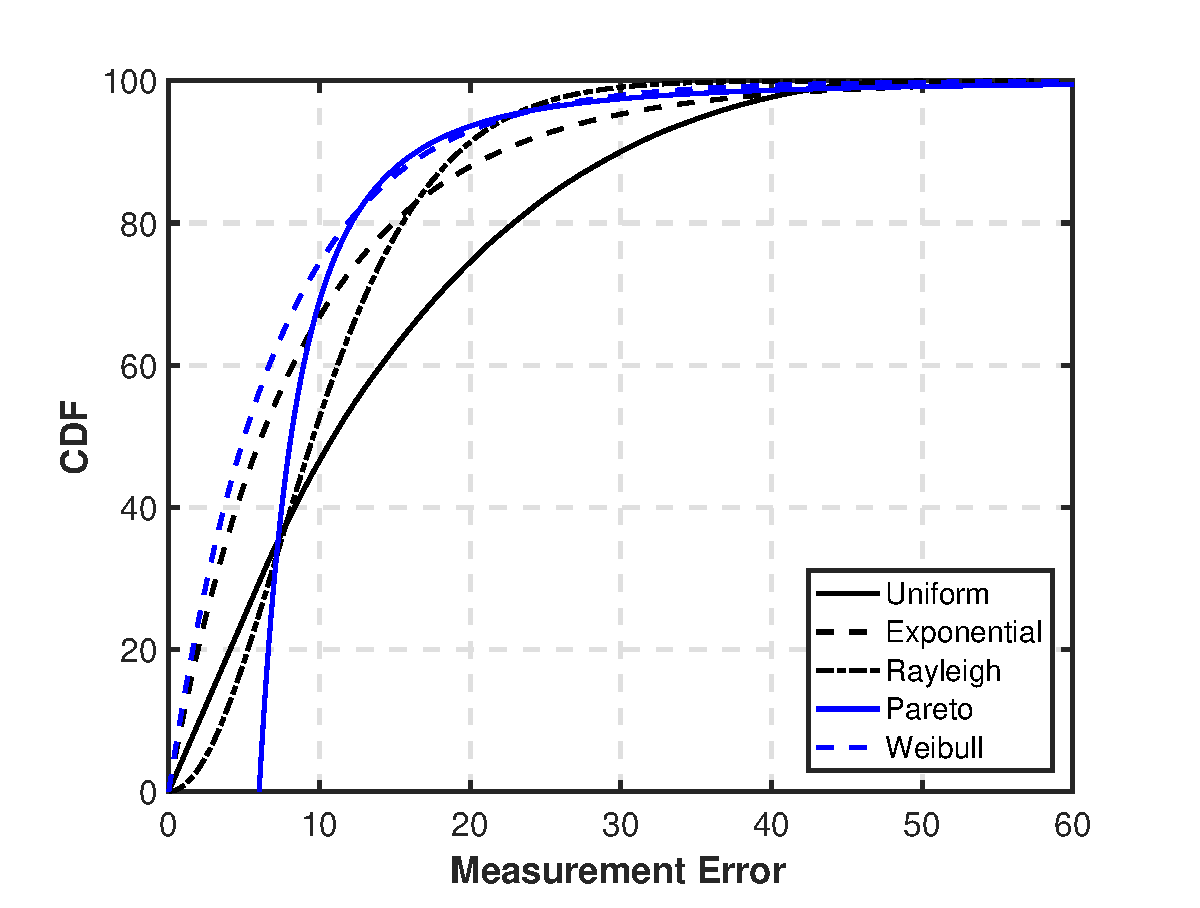
\includegraphics[width=\columnwidth]{cdf_error}
	\caption{Error CDF computed from values used in the simulations in all $1000$ Monte Carlo runs.}		
	\label{fig:cdf_error}
\end{figure}
%
%

\subsection{Simulation Results}
Figure~\ref{fig:uniform_blue_mvu} presents the performance of the three estimators when the noise is uniformly distributed in which the shaded area corresponds to $90\%$ interval of the numerical variances. Both MVU estimators, expectedly, result in noticeably less variance in the estimates compared to the BLUE estimator. It can be further observed that if the hyper parameter $b$ is unknown, the variance of the proposed estimator is negligibly larger than the case with known $b$. 
%
%
\begin{figure}[!t] 
	\centering
	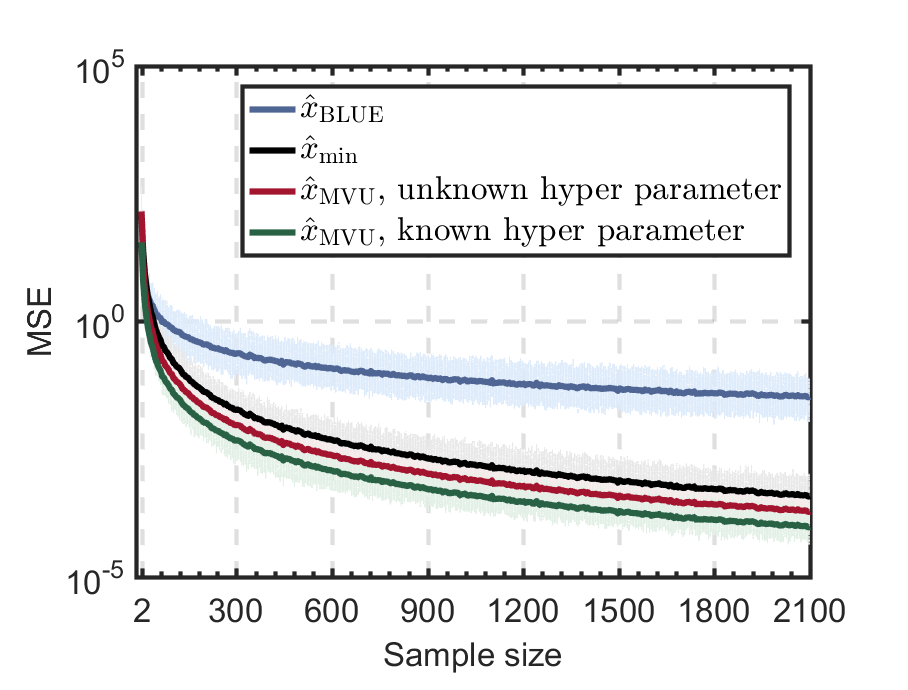
\includegraphics[width=\columnwidth]{uniform_blue_mvu}
	\caption{Analytical variance, uniform noise distribution, of BLUE, MVU with known hyperparamters, and MVU with unknown hyperparamters marked with blue, green, and red solid lines, respectively. For each estimator, the shaded are corresponds to $90\%$ interval of numerical variances obtained in simulations.}		
	\label{fig:uniform_blue_mvu}
\end{figure}
%
%
%
%
\begin{figure}[!t]
	\centering
	\subfloat[Numerical and analytical variances.]{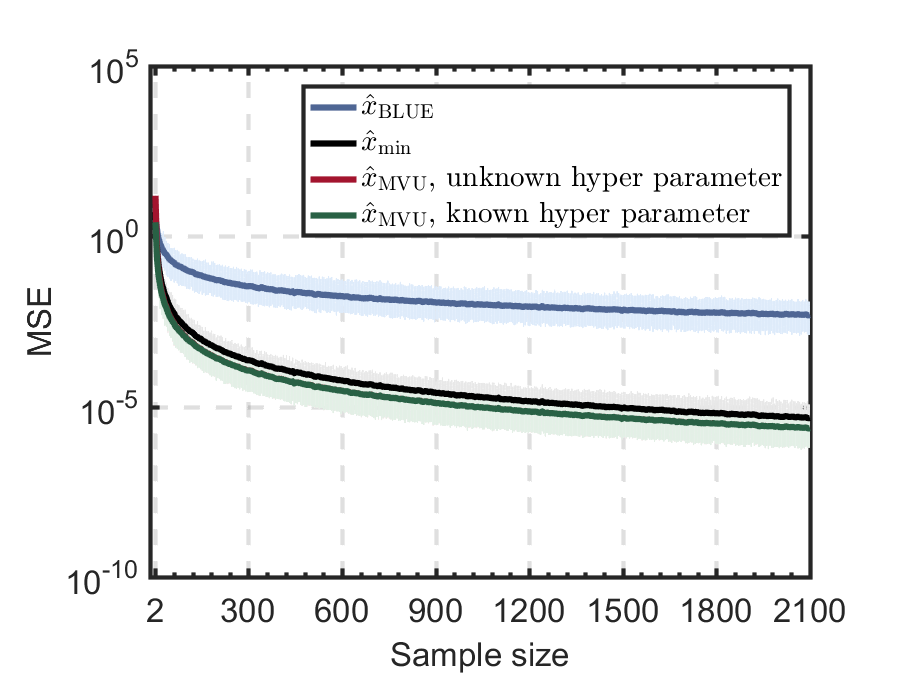
\includegraphics[width=\columnwidth]{exponential_blue_mvu}%
		\label{fig:exponential_blue_mvu_all}}
	\hfil
	\subfloat[Analytical variances for $N\leq40$.]{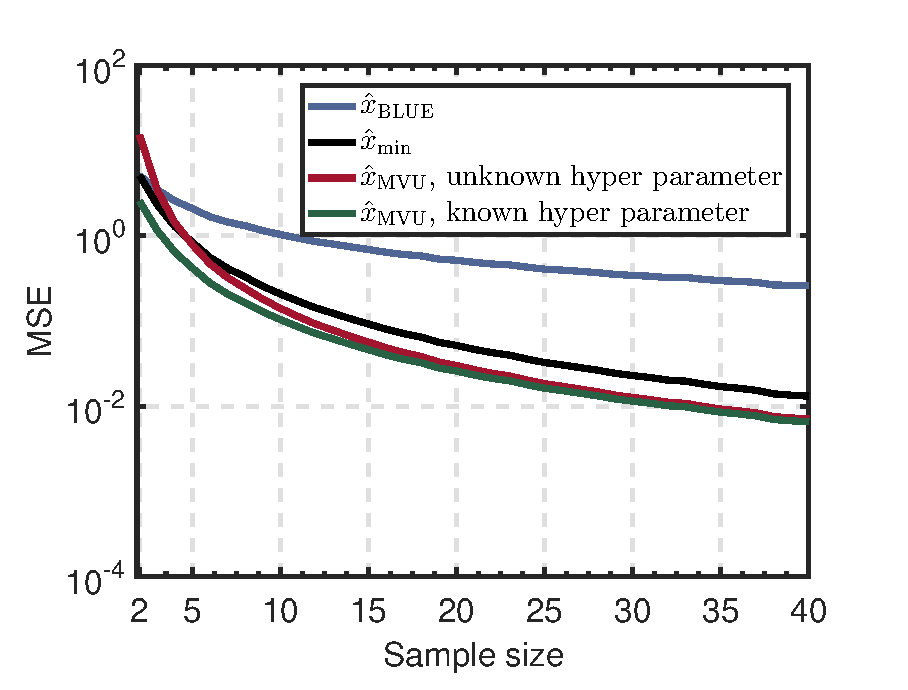
\includegraphics[width=\columnwidth]{exponential_blue_mvu_zoom}%
		\label{fig:exponential_blue_mvu_zoom}}
	\caption{Analytical variance of, exponential noise distribution,  BLUE, MVU with known hyperparamters, and MVU with unknown hyperparamters marked with blue, green, and black solid lines, respectively. For each estimator, the shaded are corresponds to $90\%$ interval of numerical variances obtained in simulations. Since the MVU estimators have similar results for large sample sizes, the analytical variances of the three estimators for smaller sample sizes are presented separately.}
	\label{fig:exponential_blue_mvu}
\end{figure}
%
%

In case of exponential noise distribution, as shown in Figure~\ref{fig:exponential_blue_mvu_all}, there is still a non-negligible different between BLUE and the two MVU estimators. However, the two MVU estimators, specially for large values of $N$, behave similarly. In order to verify their performance for smaller sample sizes, Figure~\ref{fig:exponential_blue_mvu_zoom}  illustrates the analytical variances of all the three estimators for $N<40$. At the beginning, $N\in[2,4]$ the estimator with unknown hyperparameter has the largest variance. However, for larger sample sizes, the two MVU estimators are almost equal and both have less variance than the BLUE estimator.


The BLUE and the proposed order statistic based estimator with known hyper parameter, in case of Rayleigh noise distribution, as shown in Table~\ref{tbl:estimators}, have similar variances. Hence, in this case, we only compare the BLUE estimator and order statistic estimator with unknown hyper parameter. As shown in Figure~\ref{fig:rayleigh_blue_order_all}, these two estimators have similar behavior for large data samples. However, for the smaller sample sizes,  as illustrated in Figure~\ref{fig:rayleigh_blue_order_zoom}, the BLUE (and order statistic with known hyper parameter) estimator has smaller variance compared to the case with unknown hyper parameter.
%
%
\begin{figure}[!t]
	\centering
	\subfloat[Numerical and analytical variances.]{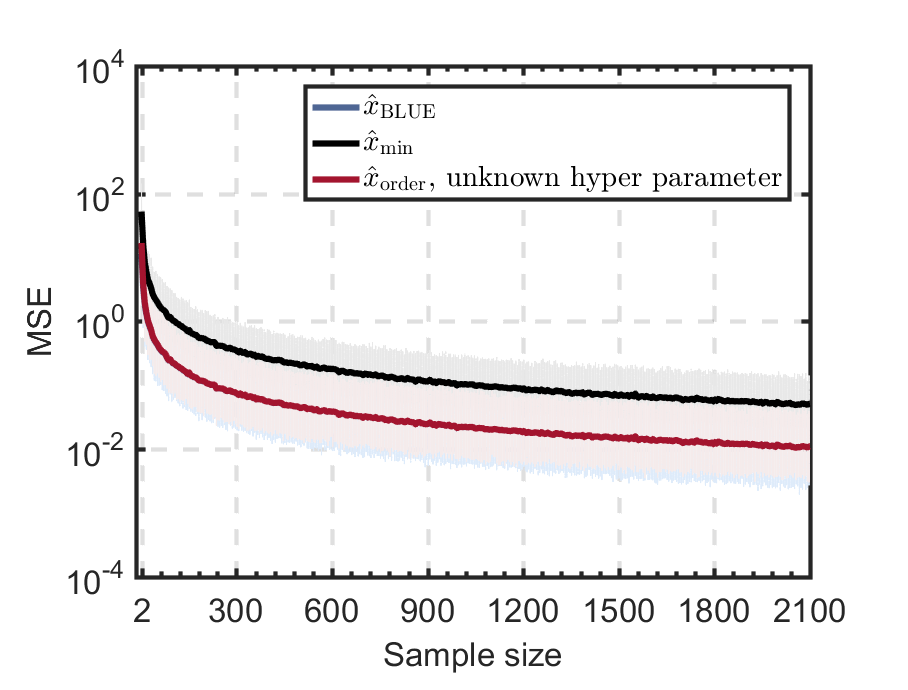
\includegraphics[width=\columnwidth]{rayleigh_blue_order}%
		\label{fig:rayleigh_blue_order_all}}
	\hfil
	\subfloat[Analytical variances for $N\leq40$.]{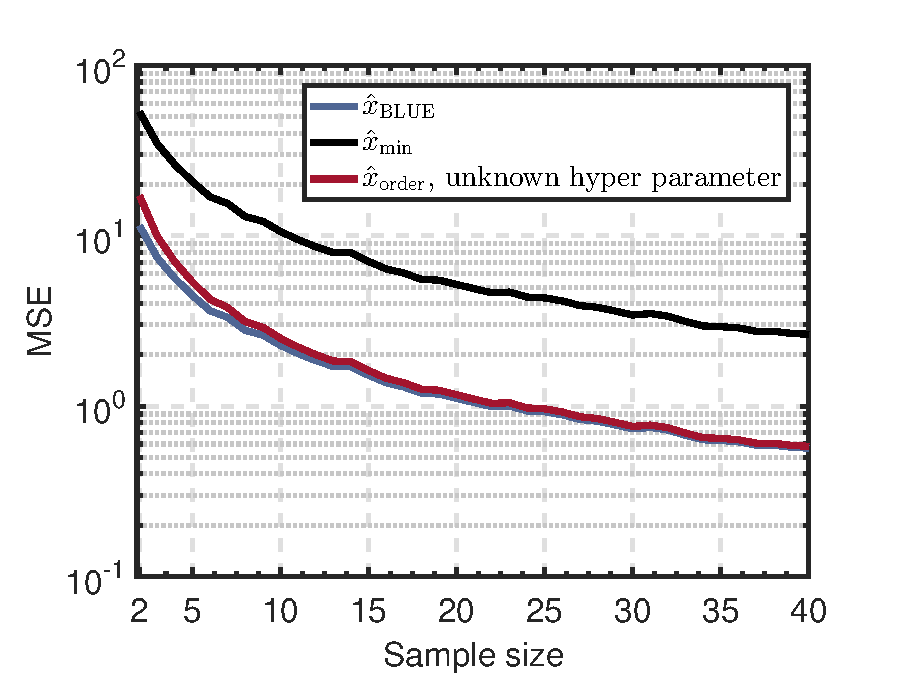
\includegraphics[width=\columnwidth]{rayleigh_blue_order_zoom}%
		\label{fig:rayleigh_blue_order_zoom}}
	\caption{Analytical variance, Rayleigh noise distribution, of BLUE and order statistic with unknown hyperparamters estimators. For each estimator, the shaded are corresponds to $90\%$ interval of numerical variances obtained in simulations. The two estimators have similar analytical results for large sample sizes, hence, the analytical variances are presented for smaller sample sizes.}
	\label{fig:rayleigh_blue_order}
\end{figure}
%
%

As Table~\ref{tbl:estimators} suggests, in case of Pareto and Weibull distributions, we only derived BLUE and an unbiased order statistic-based estimators when the two hyperparameters of the distributions are known. The two estimators for both distributions are compared and the results are presented in Figure.~\ref{fig:pareto_weibull_blue_order}. In both cases, the proposed estimator outperforms the BLUE estimator in terms of variance. 
%
%
\begin{figure}[!t]
	\centering
	\subfloat[Weibull distribution.]{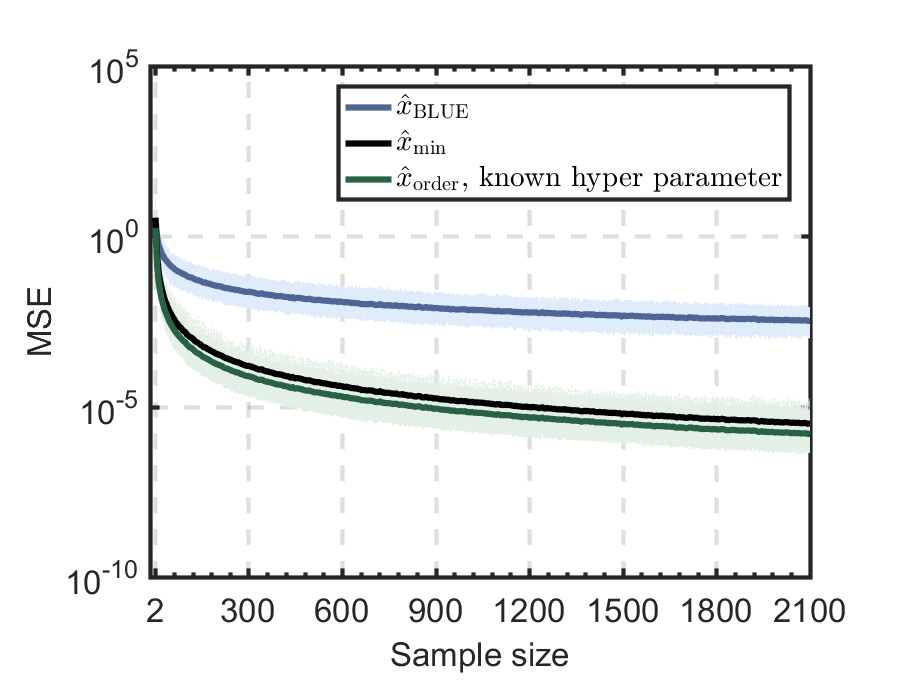
\includegraphics[width=\columnwidth]{weibull_blue_order}%
		\label{fig:weibull_blue_order}}
	\hfil
	\subfloat[Pareto distribution.]{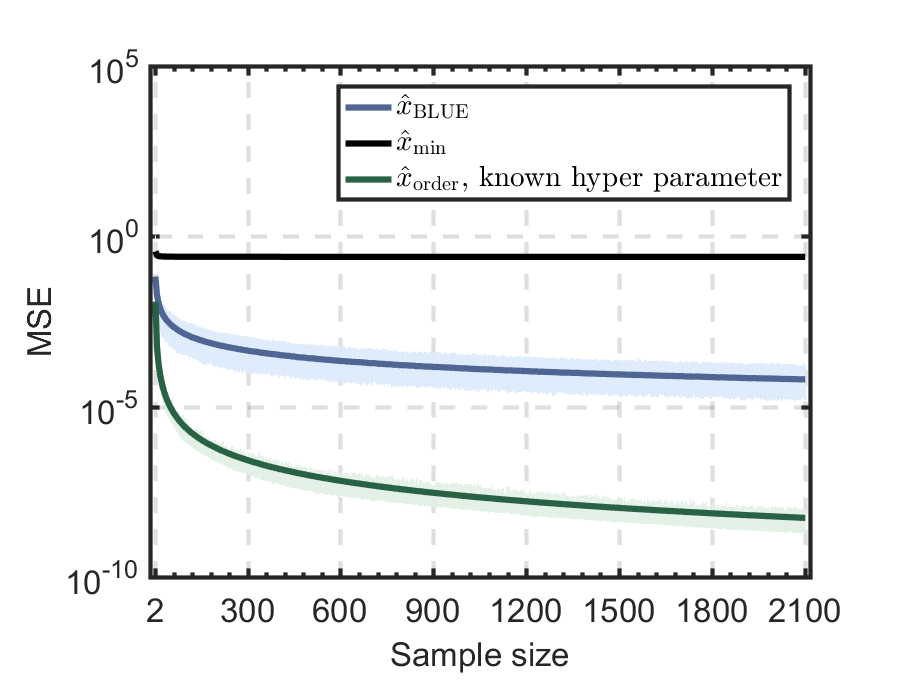
\includegraphics[width=\columnwidth]{pareto_blue_order}%
		\label{fig:pareto_blue_order}}
	\caption{Analytical variance, Weibull and Pareto noise distributions, of BLUE and order statistic with known hyperparamters estimators marked with blue and green solid lines, respectively. For each estimator, the shaded are corresponds to $90\%$ interval of numerical variances obtained in simulations.}
	\label{fig:pareto_weibull_blue_order}
\end{figure}
%
%

In case of mixture noise distribution, we consider three different scenarios based on the mixing probabilities. The CDFs of the errors for two extreme cases with dominant contribution from uniform noise,$a=0.01$, and dominant contribution from normal noise,$a=0.99$, and the case with $a=0.5$ are presented in Figure~\ref{fig:mixture_cdf}. 
%
%
\begin{figure}[!t] 
	\centering
	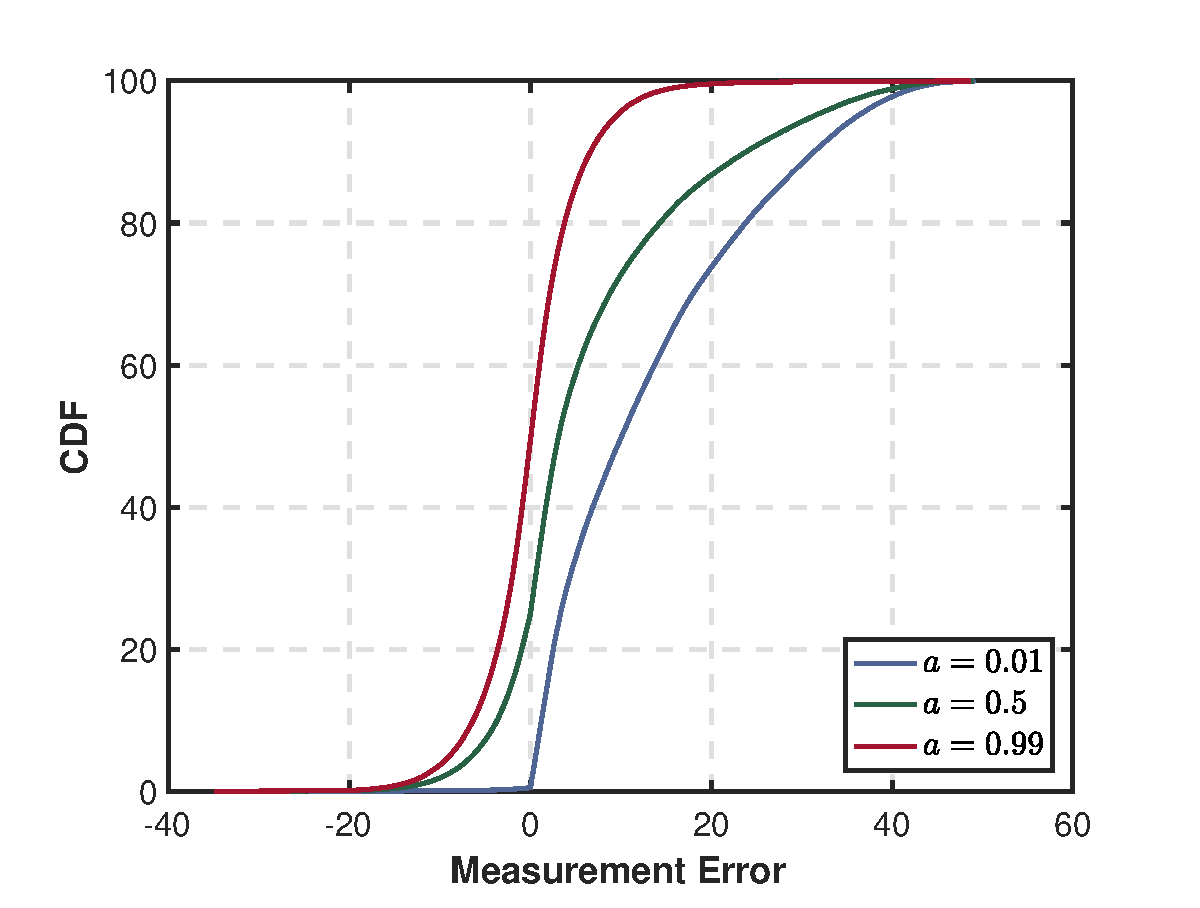
\includegraphics[width=\columnwidth]{cdf_mixture}
	\caption{Error CDF of the mixture noise $e\sim a\mathcal{N}(0,\sigma^2) + (1-a)\mathcal{U}(0,b)$ for three different values of $a$.}		
	\label{fig:mixture_cdf}
\end{figure}
%
%

In order to estimate the parameter $x_m$ in each Monte Carlo run, we sort the measurements and then find the $(\lfloor\frac{Na}{2}\rfloor+1)$:th component. Figure~\ref{fig:mixture_bias} presents the estimation bias for the three different scenarios with different mixing probabilities. As the figure suggests, in cases with $a=0.5$ and $a=0.99$, the numerical bias is almost zero even for very small sample sizes. However, for the case with $a=0.01$ the estimation bias is non-negligible. Additionally, in this case, a periodic behavior for the bias can be observed. The jumps in the biases occur exactly at pints where $\lfloor\frac{Na}{2}\rfloor+1$ switches from $k$:th measurement to $k+1$:th measurement. For instance, for $N\in[1,199]$, $\lfloor\frac{Na}{2}\rfloor=0$, hence $\hat{x}=y_{(1)}$. However, at $N=200$, $\lfloor\frac{Na}{2}\rfloor=1$, resulting in $\hat{x}=y_{(2)}$.

In the extreme case with $1\%$ contribution from normal distribution, a similar periodic pattern for the estimator's variance can also observed from Figure~\ref{fig:mixture_var} in which the solid lines represent the mean of numerical variance over $1000$ Monte Carlo runs and the shaded areas correspond to $90\%$ interval.  As a general trend for the mixture of normal and uniform noise distribution, the more contribution from normal distribution, the less variance.
%
%
\begin{figure}[!t]
	\centering
	\subfloat[bias]{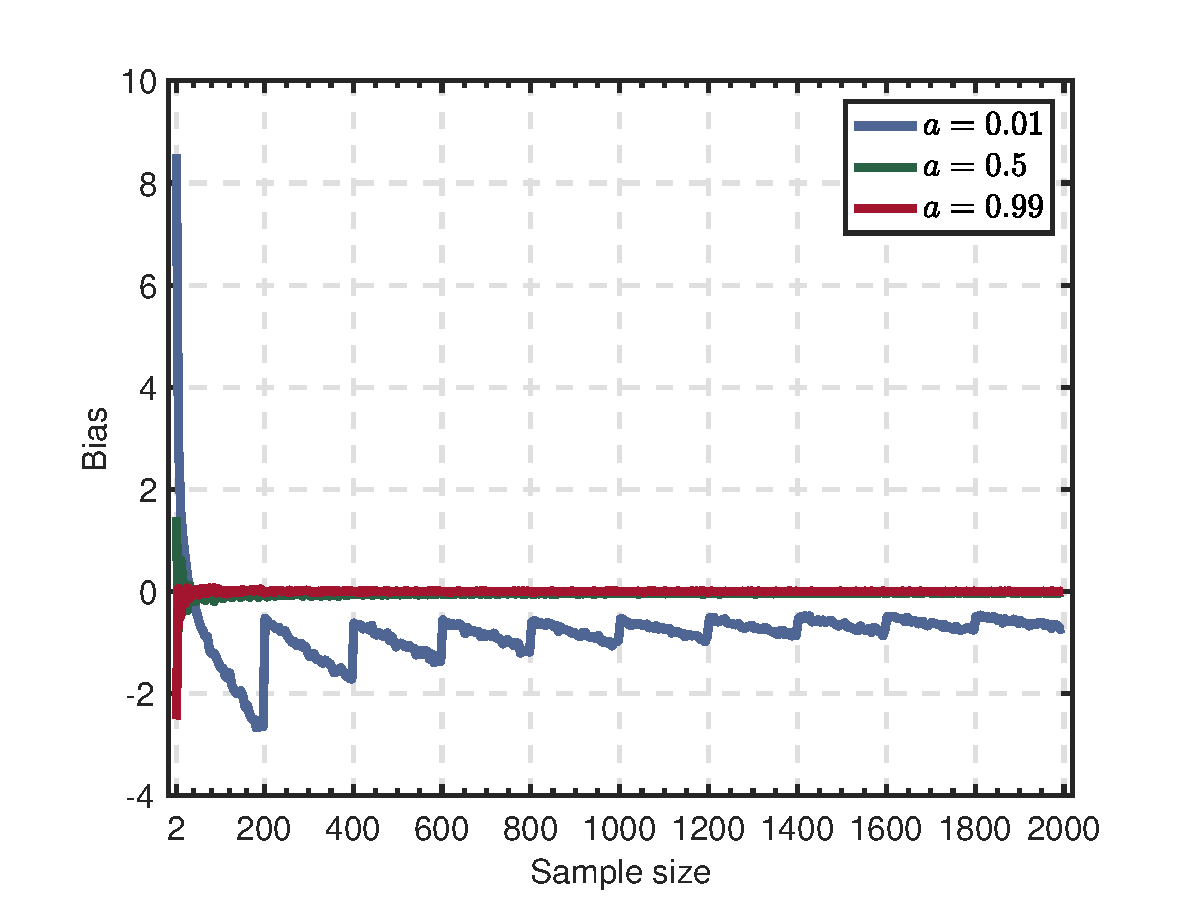
\includegraphics[width=\columnwidth]{mixture_bias}%
		\label{fig:mixture_bias}}
	\hfil
	\subfloat[variance]{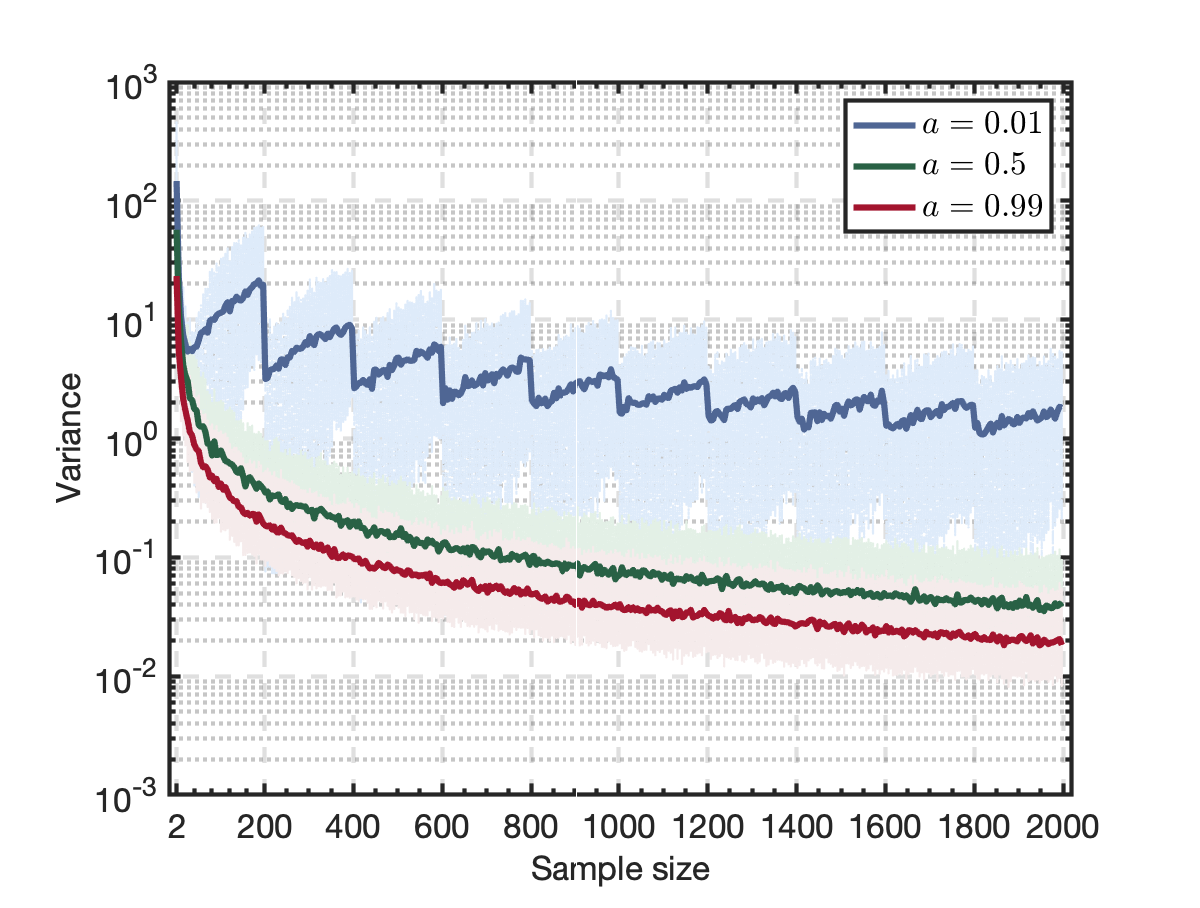
\includegraphics[width=\columnwidth]{mixture_var}%
		\label{fig:mixture_var}}
	\caption{Numerical bias and variance of the proposed order statistic estimator when the noise distribution is a  mixture of normal and uniform for different values of mixing probability $a$. }
	\label{fig:mixture_order}
\end{figure}
%
%
\section{Conclusions}\label{sec:conclusions}
In this work, the location estimation problem was studied in which an unknown parameter was estimated from observations under additive noise. Multiple noise distributions were considered and, in some cases, MVU estimators were proposed. In other cases an unbiased estimator based on minimum order statistic was derived. Furthermore, if applicable, MVU and minimum order statistic estimators without any knowledge of the hyper parameters of the underlying noise distributions were provided. The results of all the estimators were compared with BLUE in terms of variance for various measurement sample sizes. The results indicate better performance of the proposed estimators compared to BLUE, even for the case of unknown hyper parameters. Additionally, the location estimation problem under mixture of normal and uniform noise distribution was studied and the numerical variance and bias of the proposed estimator were evaluated.

\bibliographystyle{IEEEtran}
\bibliography{./ref/arxiv_18}

\end{document}


